\documentclass[12pt]{report}

% Formatting packages
\usepackage[letterpaper, margin=1in]{geometry}  % 8.5x11 paper, 1-inch margins
\usepackage{setspace}  % For spacing control

\usepackage{booktabs}
\doublespacing  % Set line spacing to double

% Font setup (IEEE recommended fonts)
\usepackage{times}  % Times font
\usepackage{mathptmx}  % Times font for math
\usepackage{longtable}
\usepackage{lscape}
\usepackage{listings}
\usepackage{xcolor}
% Additional packages
\usepackage{graphicx}  % For figures
\usepackage{amsmath, amssymb}  % Math support
\usepackage{cite}  % IEEE-style references
\usepackage{hyperref}  % Clickable links in TOC
\usepackage{acronym}  % For List of Symbols (Acronyms)
\usepackage{tocloft}  % Formatting TOC, LOF, LOT

\usepackage{subcaption} 
\usepackage{algorithm}
\usepackage{algpseudocode}
\usepackage{hyperref}

\usepackage{tocbibind}

\hypersetup{
	colorlinks=false,  % Disable colored links
	pdfborder={0 0 0}  % Remove link borders
}
\renewcommand{\listalgorithmname}{List of Algorithms}

\lstdefinestyle{mystyle}{
	backgroundcolor=\color{white},   % set background color
	basicstyle=\footnotesize\ttfamily,  % font size and family
	breaklines=true,  % automatic line breaking
	captionpos=b,  % caption position
	commentstyle=\color{green},  % comments in green
	keywordstyle=\color{blue},  % keywords in blue
	stringstyle=\color{red},  % strings in red
	numbers=left,  % line numbers on the left
	numberstyle=\tiny\color{gray},  % line number style
	stepnumber=1,  % step number for line numbering
	numbersep=5pt,  % space between numbers and code
	frame=single,  % adds a frame around the code
	rulecolor=\color{black},  % frame color
	morekeywords={def, import, yield, return, as},  % custom keywords (optional)
}
\lstset{style=mystyle}
% IEEE Reference Style
\bibliographystyle{IEEEtran}

% Customize spacing for lists
\setlength{\cftbeforesecskip}{10pt}  % Space before section entries in TOC
\setlength{\cftbeforefigskip}{10pt}  % Space before figure list
\setlength{\cftbeforetabskip}{10pt}  % Space before table list

\begin{document}
	% Cover Page
	\begin{titlepage}
		\centering
		\vspace{3cm}
		{\Huge \textbf{Automatically Identifying Action Sequences in Movies}} \\[2cm]  % Main title
		{\Large \textbf{by}} \\[1cm]  % "by" added
		{\Large Alton Lavin D'souza} \\[1cm]  % Author name
		{\Large \today} \\[4cm]  % Date
		\vfill
		% Placeholder image (replace with actual image if needed)
		% \includegraphics[width=0.5\textwidth]{placeholder.png}  % Use a placeholder or replace with a real logo
		\vfill
		
		% Required text at the bottom of the cover page
		\begin{center}
			\textit{An Engineering Project Report} \\[0.2cm]
			Submitted to the Department of Electrical \& Computer Engineering – Integrated Circuits and System Design \\[0.2cm]
			In partial fulfillment of the requirements for the degree of \\[0.2cm]
			\textbf{Master of Engineering} \\[1cm]
			Department of Electrical \& Computer Engineering – Integrated Circuits and System Design \\[0.2cm]
			University of Alberta
		\end{center}
	\end{titlepage}
	
	\pagenumbering{roman}  % Roman numeral pagination for preface
	\setcounter{page}{1}
	% Acknowledgements (New Page)
	\newpage
	\section*{Acknowledgements}
	I would like to express my sincere gratitude to Professor Cor Paul for providing me with the opportunity to undertake this project. I would also like to extend my appreciation to Professor Li Cheng and Tico Romano for their invaluable inputs and guidance throughout the course of this project. Tico Romano, in particular, was instrumental in providing the necessary domain knowledge and dataset for this work, and his blogs were a crucial resource that greatly influenced the direction and execution of the project.
	
	My sincere thanks go to the members of the Asgaard Lab for their technical support, which greatly contributed to the success of this work. Lastly, I would like to thank Abhishek Sharma for his assistance and help during the project. Without their support, this project would not have been possible.
	% Abstract Section (New Page)
	\newpage
	\section*{Abstract}
	\fontsize{12}{15}\selectfont  % Increase font size
	\noindent % Avoid indent on first line
	This project aims to develop a pipeline for automatically identifying action sequences in movies, which is a time-consuming and labor-intensive when performed manually. Our approach integrates Shot Boundary Detection (SBD), Key Shot Extraction (KSE), and Visual Question Answering (VQA) using Vision-Language Models (VLMs) to automate this process. We compare our novel SBD method against existing techniques, particularly Autoshot, which is optimized for short-form media, and demonstrate its effectiveness for long-format content like movies.
	
	For SBD, we leverage Sigmoid Loss for Language-Image Pre-training (SigLIP) to extract video frame features and employ cosine similarity to detect shot boundaries, analyzing the impact of different similarity thresholds on detection accuracy. Additionally, we explore the role of KSE in improving video annotation efficiency, particularly in resource-constrained scenarios. Finally, we evaluate the effectiveness of zero-shot video annotation and supervised fine-tuning of a VLM for automated video annotation. This work contributes to enhancing automated video analysis, making large-scale film indexing and annotation more practical. Our results show that an optimum cosine similarity threshold lies between 0.8 and 0.85 and provided you have good data Supervised Fine-tuning will help achieve better results than trying to prompt engineer with zero-shot methods.
	
	\begingroup  % Start group to suppress ToC entries
	\renewcommand{\addcontentsline}[3]{}
	% Table of Contents (New Page)
	\newpage
	\tableofcontents  % Generates a table of contents
	\newpage
	
	% List of Figures (New Page)
	\listoffigures
	\newpage
	
	% List of Tables (New Page)
	\listoftables
	\newpage
	
	% List of Symbols (New Page)
	\section*{List of Symbols}
	\begin{acronym}
		\acro{CNN}{Convolutional Neural Network}
		\acro{AI}{Artificial Intelligence}
		\acro{ML}{Machine Learning}
		\acro{SBD}{Shot Boundary Detection}
		\acro{KSE}{Key Shot Extraction}
		\acro{KFE}{Key Frame Extraction}
		\acro{SME}{Start Mean Error}
		\acro{EME}{End Mean Error}
		\acro{ASD}{Action To Story Duration}
		\acro{Action to Act Duration}{AAD}
		\acro{HAR}{Human Action Recognition}
		\acro{SVM}{Support Vector Machine}
		\acro{OCR}{Optical Character Recognition}
		\acro{T.V.}{TeleVision}
		\acro{SVR}{Support Vector Regression}
		\acro{DFW}{Dynamic Frame Wrapping}
		\acro{3D}{Three Dimensional}
		\acro{C3D}{Convolutional 3D models}
		\acro{LSTM}{Long Short Term Memory}
		\acro{TAM}{Temporal Aggregation Module}
		\acro{TSM}{Temporal Shift Module}
		\acro{RGB}{Red Green Blue}
		\acro{ST-GCN}{Spatio Temporal-Graph Convolutional Network}
		\acro{LLM-AR}{Large Language Model as an Action Recognizer}
		\acro{LLMs}{Large Language Models}
		\acro{CT}{Cut Transition}
		\acro{GT}{Gradual Transition}
		\acro{ResNet}{Residual Network}
		\acro{GPU}{Graphics Processing Unit}
		\acro{SigLIP}{Sigmoid Loss for Language Image Pre-Training}
		\acro{CUDA}{Compute Unified Device Architecture}
		\acro{LLaVA}{Large Language and Vision Assistant}
		\acro{LoRA}{Low Rank Adaptation}
		\acro{QLoRA}{Quantized Low Rank Adaptation}
		\acro{SFT}{Supervised Fine-Tuning}
	\end{acronym}
	\newpage
	\listofalgorithms 
	\endgroup 
	
	\newpage
	\pagenumbering{arabic}  % Switch to Arabic numerals
	\setcounter{page}{1}
	
	% Introduction (New Page)
	\newpage
	\chapter{Introduction}
	\cite{tico-romao-2024} Action identification in action movies refers to the process of recognizing key action moments in films. Historically, action films feature seven recurrent scenarios: rescue, escape, capture, heist, fight, pursuit, and speed. Additionally, there are other scenarios, such as transfer, where a character moves from one mode of transport to another. However, transfer scenarios are not as historically prominent as the other aforementioned scenarios. We can see transfer scenarios prominent in movies like "The Fast and the Furious (2011)" and "Carter (2022)". 
	 
	Two key aspects of note while dealing with action films are action moments and action scenarios. Action moments deals with the temporal aspects of actions in films while action scenarios deals with the spatial aspect of actions.
	
	Action types can be categorized based on the number of defining features: low typicality and high typicality. Low typicality actions exhibit only a few defining features, whereas high typicality actions display a large number of features. A common pattern observed in action sequences is a transition from high typicality to medium and then to low typicality, which is referred to as the typicality gradient. For instance, in a fight scene, the action typically involves two opposing parties—either a one-on-one duel or a clash between two combat forces. An example of a one-on-one fight scene is shown in Figure~\ref{fig:bond}, depicting a scene from From Russia with Love (1963), where James Bond and Red Grant engage in combat aboard the Orient Express. Figure~\ref{fig:saving_private_ryan} shows an example of a high typicality fight scene from the movie "Saving Private Ryan (1998)" where we see mulitiple soldiers landing on the beach of Normandy on D-Day under a hail of bullets. Figure~\ref{fig:red_dawn} and Figure~\ref{fig:logan} show examples of low and medium typicality which is characterized by scenes of one sided aggression. The difference between the two typicalities is the intensity of action or motions in the scenes.
	
	In the next few sections, we are going to see how such actions are isolated and how isolating such action moments can be subjective and why an automated solution is needed to help isolate action moments uniformly.
	
	
	
	\begin{figure}[h]
		\centering
		\begin{minipage}{0.45\linewidth}
			\centering
			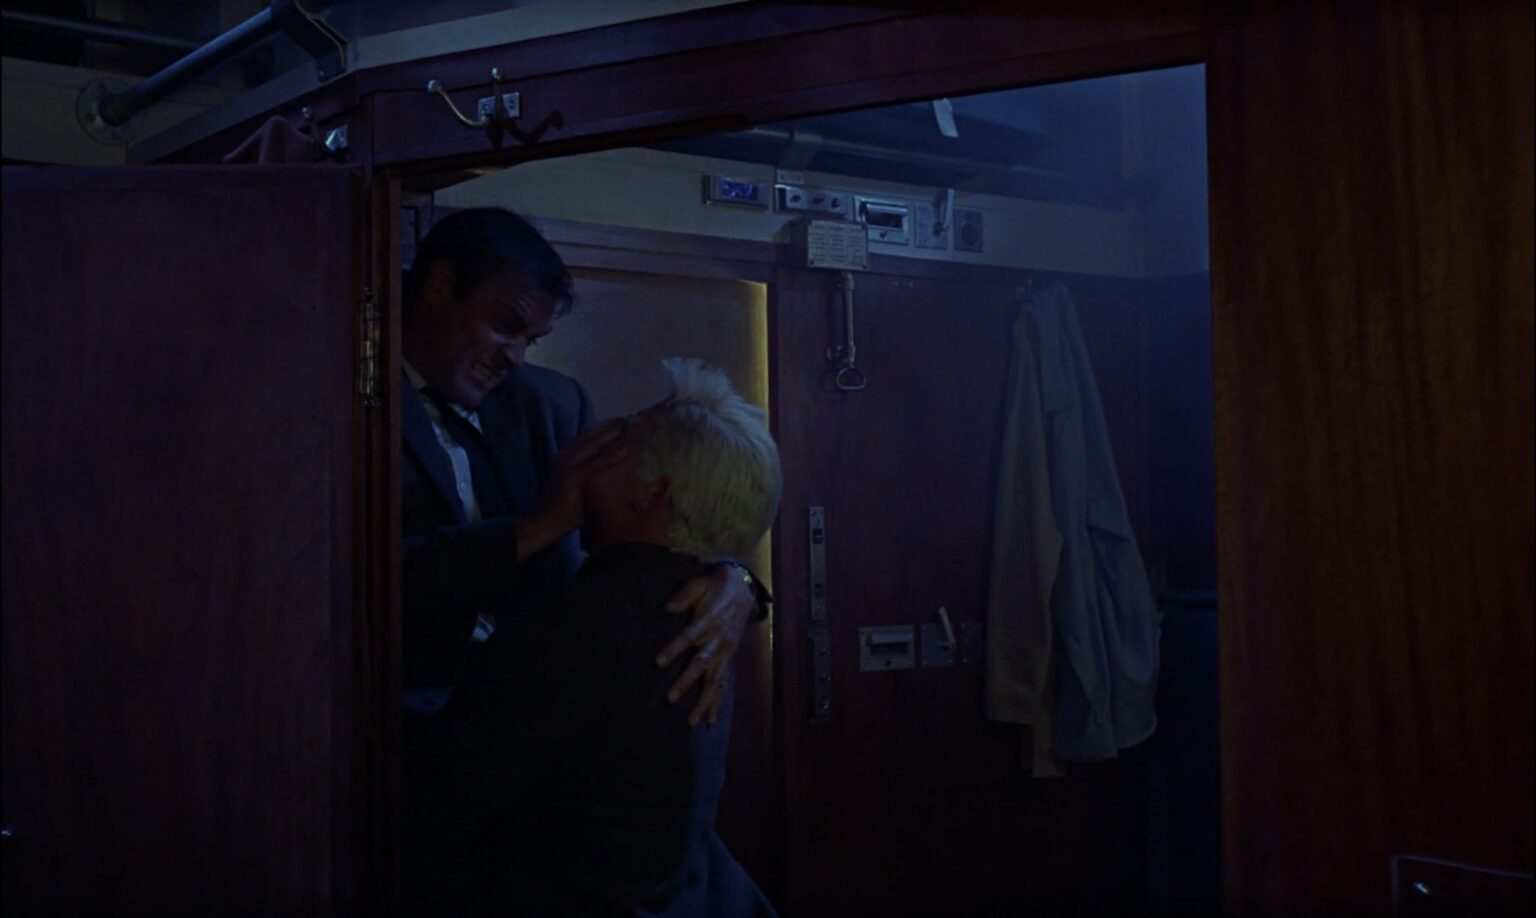
\includegraphics[width=\linewidth]{From-Russia-with-Love-1963.jpg}
			\caption{One-on-One fight scene in the movie "From Russia with Love (1963)" (High typicality) \cite{tico-romao-2024}}
			\label{fig:bond}
		\end{minipage}
		\hspace{0.05\linewidth}  % Space between the figures
		\begin{minipage}{0.45\linewidth}
			\centering
			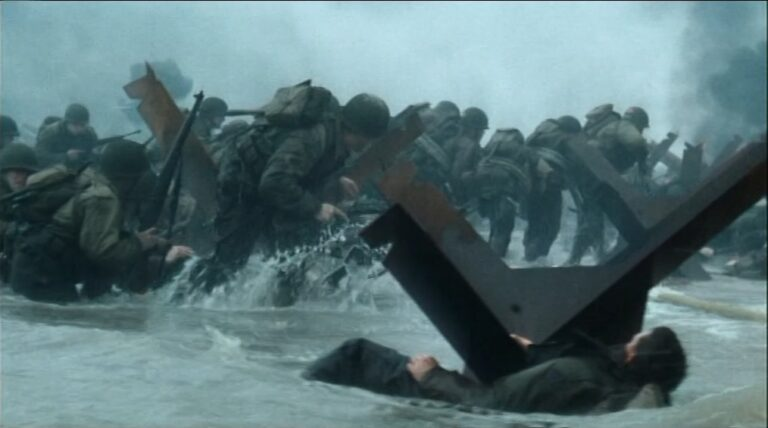
\includegraphics[width=\linewidth]{Saving-Private-Ryan-1998.jpg}
			\caption{Multi-participant fight in the film "Saving Private Ryan (1998)" (High typicality)\cite{tico-romao-2024}}
			\label{fig:saving_private_ryan}
		\end{minipage}
	\end{figure}
	
	
	\begin{figure}[h]
		\centering
		\begin{minipage}{0.45\linewidth}
			\centering
			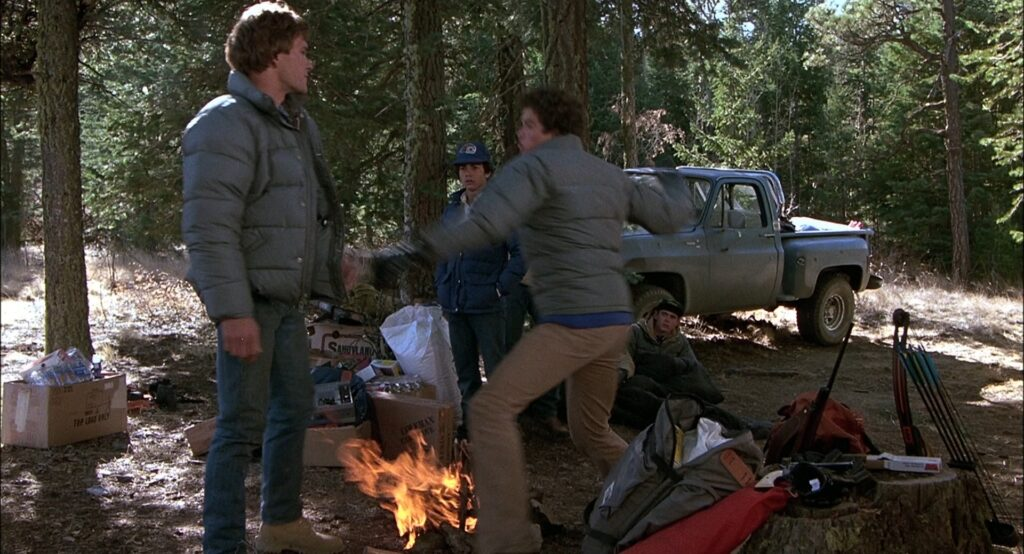
\includegraphics[width=\linewidth]{Red-Dawn-MT-1984.jpg}
			\caption{A scene of one sided act of aggression in the movie "Red Dawn (1984)" (Medium Typicality)  \cite{tico-romao-2024}}
			\label{fig:red_dawn}
		\end{minipage}
		\hspace{0.05\linewidth}  % Space between the figures
		\begin{minipage}{0.45\linewidth}
			\centering
			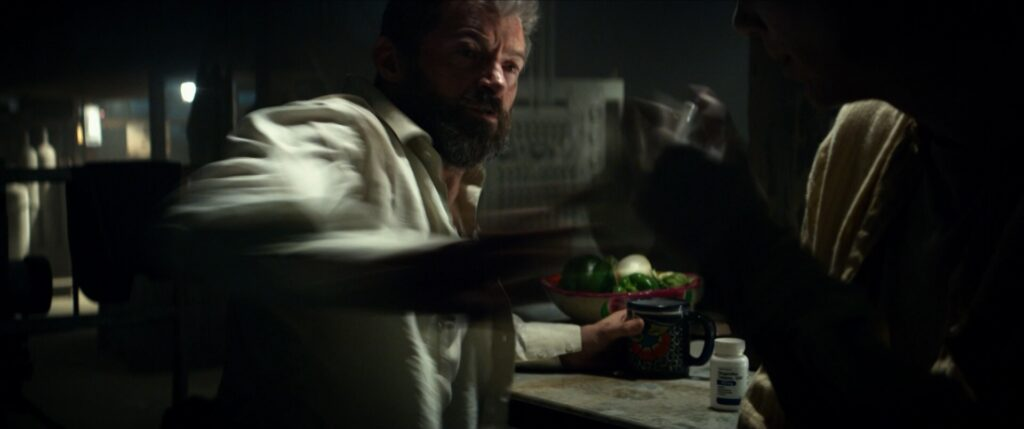
\includegraphics[width=\linewidth]{Logan-LT-2017.jpg}
			\caption{A one sided aggression scene from "Logan (2017)"(Low Typicality)\cite{tico-romao-2024}}
			\label{fig:logan}
		\end{minipage}
	\end{figure}
	
	\section{Isolating Action Moments in Film}
	A typical workflow according to \cite{tico-romao-2024} while annotating action moments in movies is to first identify them, measure the duration and take note of the action combinations involved in a scene. Typical manual workflow involved while performing this process is to cut a section of the film just before the action commences as the start point and to cut it again after the action has ended. The length of the clip from the start to end of the cut is known as the action duration or action moment. An action moment can be as short as 3 seconds and can be as long as 44 minutes. The next step in the process is to identify the combination of actions present in the action moments.
	
	\section{Presence of Multiple Action Scenarios}
	In an action moment there are usually multiple action scenarios. These action scenarios occur either sequentially, which is known as a horizontal combination of action scenarios or concurrently, which is a known as a vertical combination of action scenarios. Examples of each combination is shown in Figure 
	 which shows some vertical and horizontal combination of action scenarios in the film "Bonnie and Clyde (1967)"
		\begin{figure}[h]
		\centering
		\begin{minipage}{0.45\linewidth}
			\centering
			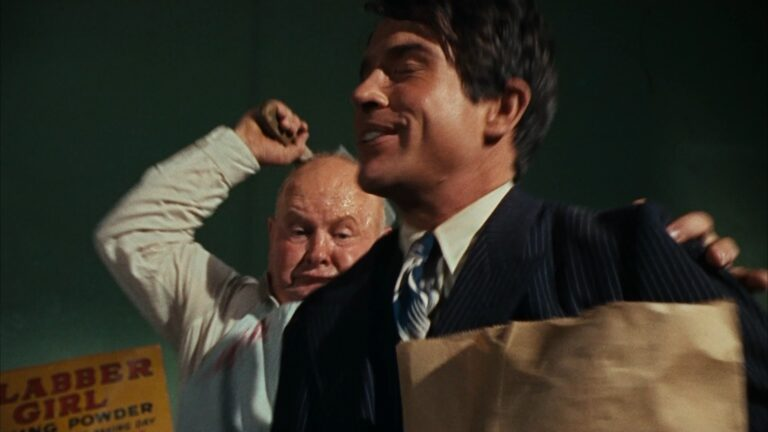
\includegraphics[width=\linewidth]{Bonnie-and-Clyde-R2-1967-768x432.jpg}
			\caption{ Heist and fight scenarios happening concurrently in "Bonnie and Clyde (1967)" (Vertical Combination) \cite{tico-romao-2024}}
			\label{fig:bonnie_and_clyde_1}
		\end{minipage}
		\hspace{0.05\linewidth}  % Space between the figures
		\begin{minipage}{0.45\linewidth}
			\centering
			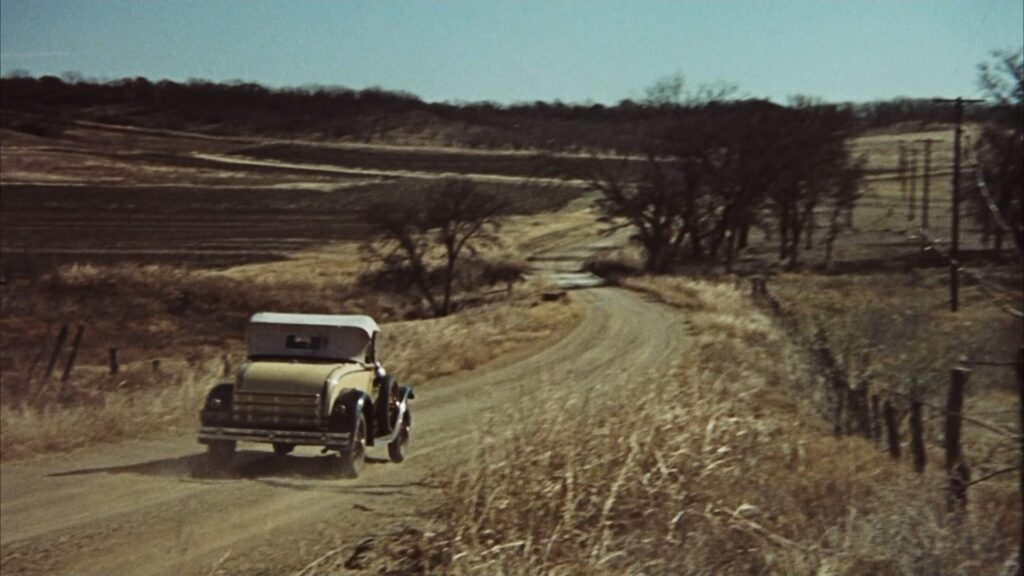
\includegraphics[width=\linewidth]{Bonnie-and-Clyde-R4-1967-1024x576.jpg}
			\caption{Heist and scenarios happening sequentially in "Bonnie and Clyde (1967)" (Horizontal Combination) \cite{tico-romao-2024}}
			\label{fig:bonnie_and_clyde_2}
		\end{minipage}
	\end{figure}
	% Methodology (New Page)
	\section{Data Collation}
	After capturing action moments and annotating them with the appropriate action scenarios, we proceed to calculate the Action to Story Duration (ASD) Ratios and Action to Act Duration (AAD) Ratios. Capturing action moments and action scenarios helps us build an action profile which typically has the following attributes:
	
	\begin{enumerate}
		\item Duration of the film - The entire duration of the movie in question
		\item Action time or film duration ratio - This is the ratio of total duration of various action scenarios to the duration of the film
		\item Act Start - Start of an Act in a movie which might have on or more acts
		\item Act End - End of an Act which might align to the start of the next act.
		\item Act Duration - the duration of an Act which is essentially $Act\,Duration = Act\,End - Act\,Start$.
		\item Action Sequences - This is the title given to a series of actions that are taking place with in an Act. For example, Rambo's Escape and Hunting Rambo are titles given to action sequences that correlate with title itself.
		\item Participants - These are characters involved in an action sequence.
		\item Narrational Perspectives - The point of view from which a character witnesses or experiences the action sequences in the film.
		\item Action Forms - The various action scenarios occurring within an action sequence.
		\item Act - \cite{chris-baldwin} An act is the part of movie defined by theatrical elements like action, climate and resolution. In this scenes are grouped into Acts based on actions.
		\item Start - The start of an action sequence
		\item End - The end of an action sequence
		\item Duration - The duration of an action sequence which can typically be calculated by $Duration = End - Start$
	\end{enumerate}
	
	The action profile is necessary to better understand the structure of an action film and the genre itself. For this project, the  focus is on identifying action forms. Action Form Identification might seem similar to human action recognition (HAR), which is not the case the difference lies in the features being tracked. In HAR only people are being tracked while in action form identification multiple aspects are being tracked i.e. objects in a film like car, tempo of the film and people as well. However, we can still leverage techniques used for HAR in identifying action forms. These techniques extract the spatial and temporal features of video and can be used for action form identification. In the next section we will see some related works on not only HAR, but also action form identification as well.
	\chapter{Related Works}
	
	In this section we will see a lot of literature on extracting spatial temporal feature for action recognition. Some of these can be repurposed for action form identification.
	
	\cite{h_w-chen} In the paper by H.W. Chen et. al. some work has been done around action movie segmentation and summarization based on the tempo of scenes, which is the speed of delivery of segments of movies. They leverage domain knowledge, shot change detection, motion activity analysis and audio feature extraction to understand the tempo of movie segments which helps in the process of automated action movie segmentation and summarization. The tempo of the movie is computed using all the aforementioned features using the Tempo Computation formula, which helps quantify the tempo of movie shots. Using the formula from the Tempo Computation formula, the authors rank shots to perform movie segmentation and summarization. For segmentation they make use of a hierarchical clustering algorithm proposed by Zhang et. al. \cite{zhang}, but for both tasks the same process is followed wherein we first rank shots based on tempo, then based on the high tempo shots we select a shot boundary around these shots. Movie Summarization i.e. trailers and previews are created by concatenating shots based on ranks, for trailers all the high tempo shots are compiled and added to the trailer, while for previews within a group of shots or rather story units we select the top tempo shots and shots before and after this shot and add these shots to the preview of the movie in question.
	
	\cite{i-laptev} I. Laptev et. al. paper addresses the concern of lack of dataset when it comes to human action recognition in movies. In order to create a model or method to learn human action in movies the authors introduce an automated method of creating a dataset for learning human actions. To create the dataset the authors first collect relevant movie scripts which are typically publicly available and then perform script alignment. Script alignment is the process matching the temporal information of the script and movie. The scripts provides information like description of scenes, characters, dialogs and human actions. The authors use this information to retrieve human actions from the script. Anticipating that there will be some degree of misalignment, the authors come up with an alignment score to correct for the error. The authors found that only 70\% data was correctly aligned. The next step in the pipeline was to extract the action in the script, the authors chose a text classifier, which is a machine learning model that uses bag of words to perform sentiment analysis. They use a model that is quite similar to SVM.
	
	\cite{gaidon}A. Gaidon et. al. proposes a system that classifies the video clips into 6 classes of actions such as walk, fall, punch, kick, kiss and get up. The proposed system first starts by extracting the subtitles. In this case the subtitle information for the T.V. series "Buffy the Vampire Slayer" is composed as an image. To extract the subtitle information from the video frames, the authors rely on Tessract OCR. This process rarely produces any error. The authors then align the subtitle with the transcript so that it's easy to extract the temporal information. Using this aligned transcript the authors use a grammar parser to extract verbs, these verbs are used to annotate and extract video clips containing an action. Video sequences are represented in the same method as discussed in the work done by  I. Laptev et. al.. To fix inconsistent annotated video clips the authors propose to use ranking methods for visual consistency, they found that using a weakly supervised method like iterative SVR is best suited for the task.
	
	\cite{kulkarni} K. Kulkarni et. al. propose a solution for continuous action recognition wherein classification and segmentation. Segmentation in this context should not be mistaken for image segmentation, but segmentation in video clips instead. The authors devise a novel technique known as dynamic frame warping (DFW). Two implementations of the technique was proposed i.e. One pass DFW and Two Pass DFW. The first step in DFW is to create an action template for each category of an action. The purpose of this template is to caption inherent variabilities of an action. Using the action templates the authors create a super template that combines all the action templates in any random order, each video frame is then represented by a high dimensional feature vector. A window is chosen in such a way that its center is centered on each frame and to ensure there are minimum number of features to work with. The authors then calculate the frame to metaframe dissimilarity which helps align the test video sequences with action templates while also accounting for any variability.
	
	\cite{c_f_chen} The paper by C.-F. Chen et al. is a survey of 2D and 3D CNN based models for spatio-temporal feature extraction. Some key findings by the authors are: (1) The choice of backbone architecture greatly influences the performance of the model. The authors found that using ResNet50 as the backbone produced the best outcomes. (2) Temporal Pooling is found to be effective on some datasets. Temporal Pooling is the process of aggregating information across multiple frames. (3) Simple temporal aggregation methods like Temporal Aggregation Module(TAM) and Temporal Shift Module(TSM) can outperform complex models that emphasize the need for efficient temporal modeling strategies.
	
	\cite{g-yao} G. Yao et. al. survey various CNN based methods and categorize them based on the way they process data: (1) Single Channel CNN, Processes video data as a single input stream extracting spatio-temporal features from the entire video sequence. Some models that fall under this category are 3D CNN models and Convolutional 3D models (C3D). (2) Dual Channel CNN, this method processes the spatial features and temporal features separately and hence, require two separate CNN channel for processing. The models that fall under this category are 2 stream CNN models and CNN+LSTM models. (3) Fusion based approaches, this approach combines various CNN architectures and traditional methods to improve feature extraction and action recognition.
	
	\cite{manakitsa} In the paper "A review of Machine Learning for Object Detection, Semantic Segmentation and Human Action Recognition in Machine and Robotic Vision", the authors showcase how various methods like RGB-based and skeleton-based approaches are used for human action recognition. RGB based methods rely on visual data from video frames and have evolved significantly. A foundational CNN based approach that is widely used to extract spatial and temportal features are Two-Stream 2D CNNs. Additionally, the authors have found that a combination of RNN and CNN  based approaches produce good outcomes, since they are good at recognizing complex temporal patterns. The dawn of 3D CNNs which are essentially an extension of 2D CNNs allow for simulataneous modeling of spatial and temporal features. Transformer networks have recently been adopted for their ability to not only model long range dependencies but also for their processing speed.  Some known networks are the Video Transformer Networks and Interpretability Aware Redundancy Reduction Network. Unlike RGB based methods, skeleton based methods track the geometric structure of human joints. Like RGB based methods, skeleton based methods include CNN and RNN based implementation and sometimes include a combination of both methods. It was also found that Graph Convolutional Networks like ST-GCN are good at tracking the skeleton structure for action recognition. In some cases, the authors have found that combining RGB and skeleton based approaches mitigated their individual shortcomings, this method is known as multimodal fusion.
	
	\cite{llms} H. Qu et. al. in their paper propose a novel framework called Large Language Model as an Action Recognizer (LLM-AR) which is used for skeleton based human action recognition. LLMs are typically used for Natural Language Processing tasks, to make the process of skeleton based action recognition compatible with LLMs, the authors introduce a process called linguistic projection that converts skeleton sequences into a text-like format called action sequences, which can then be processed by an LLM for classification.
	
	
	
	
	
	
	
	
	
	
	

	\newpage
	\chapter{Methodology}
	In this section we will propose a pipeline and provide the details of components involved in the pipeline and the experiments carried out to implement these components.
	\begin{figure}[h]  % "h" places it approximately here
		\centering
		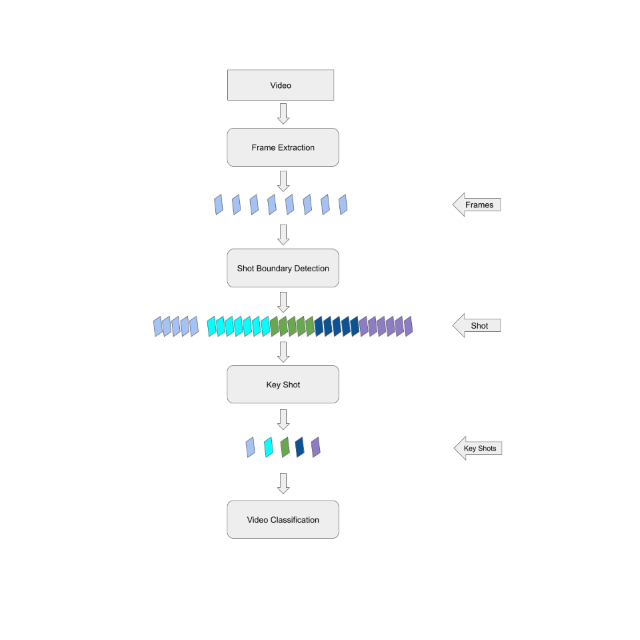
\includegraphics[width=\linewidth]{entire_pipeline.png}  % Adjust width as needed
		\caption{Illustration of the proposed pipeline for identifying films}
		\label{fig:entire_pipeline}
	\end{figure}
	\section{Proposed Approach}
	Our proposed system has the following components:
	\begin{enumerate}
		\item Shot Boundary Detection (SBD)
		\item Key Shot Extraction (KSE)
		\item Shot Classification
	\end{enumerate}
	\subsection{Shot Boundary Detection (SBD)}
	\cite{sbd} Shot Boundary Detection (SBD) also known as shot segmentation is the process of extracting features from frames of a videos and then classify the frame i.e. detecting the shot type by understanding the difference in features among various shot types. There are two types of shots detection: (1) Cut Transition (CT) and Gradual Transition (GT). However, accuracy of various shot boundary detection algorithms is hindered by presence of certain effects in video shots like variations in intensity of light and object orientation . Additionally, camera operations such as zooming, panning and tilting can hinder shot boundary detection algorithms.
	
	A video can be broken down into 3 main hierarchies: a scene, shot and a frame, as illustrated in  figure~\ref{fig:video_decomposition}. A scene is a logical grouping of shots in a story unit, whereas a shot is a series of frames captured without any cuts. A frame forms the smallest unit in a video.
	
	There are two types of transitions: (1) Cut and (2) Gradual. A cut is a drastic change in scenery from one frame to another, while a gradual transition is a change in the same scenery that happens over several frames. Depending on the way the scenery changes, gradual transitions can further be classified into fade in, fade out,  dissolve, wipe. Examples of such transitions are given in figures~\ref{fig:fade_out},~\ref{fig:fade_in},~\ref{fig:dissolve} and ~\ref{fig:wipe}. It should be noted most algorithms have a tough time detecting wipes and dissolves. 
	
	The best Deep Learning-based model for shot boundary detection according to the CLIPShots benchmark is Autoshot. However, it is only used to detect cut transitions and not gradual transitions. The algorithm we propose uses a pre-trained model like \cite{siglip} SigLIP to extract the features of individual frame in the form of a feature vector. We use a window of size 2 and extract the features of video frames i.e.  frame $n$ and frame $n+1$ within this window and then compute the cosine similarity. If the similarity falls below a certain threshold $\tau$ we classify  frame $n$ as the shot boundary. The same algorithm is described in Algorithm~\ref{alg:shot-detection} and Figure~\ref{fig:sbd_illustration}
	
	\begin{figure}[h]  % "h" places it approximately here
		\centering
		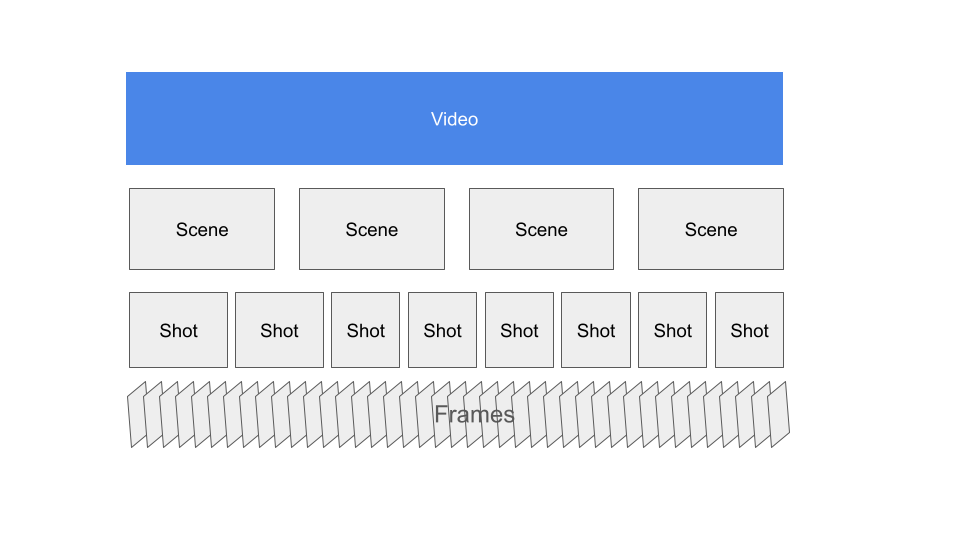
\includegraphics[width=\linewidth]{video_decomposition.png}  % Adjust width as needed
		\caption{Video Hierarchy \cite{sbd}}
		\label{fig:video_decomposition}
	\end{figure}
	
	
	\begin{figure}[h]
		\centering
		\begin{minipage}{0.45\linewidth}
			\centering
			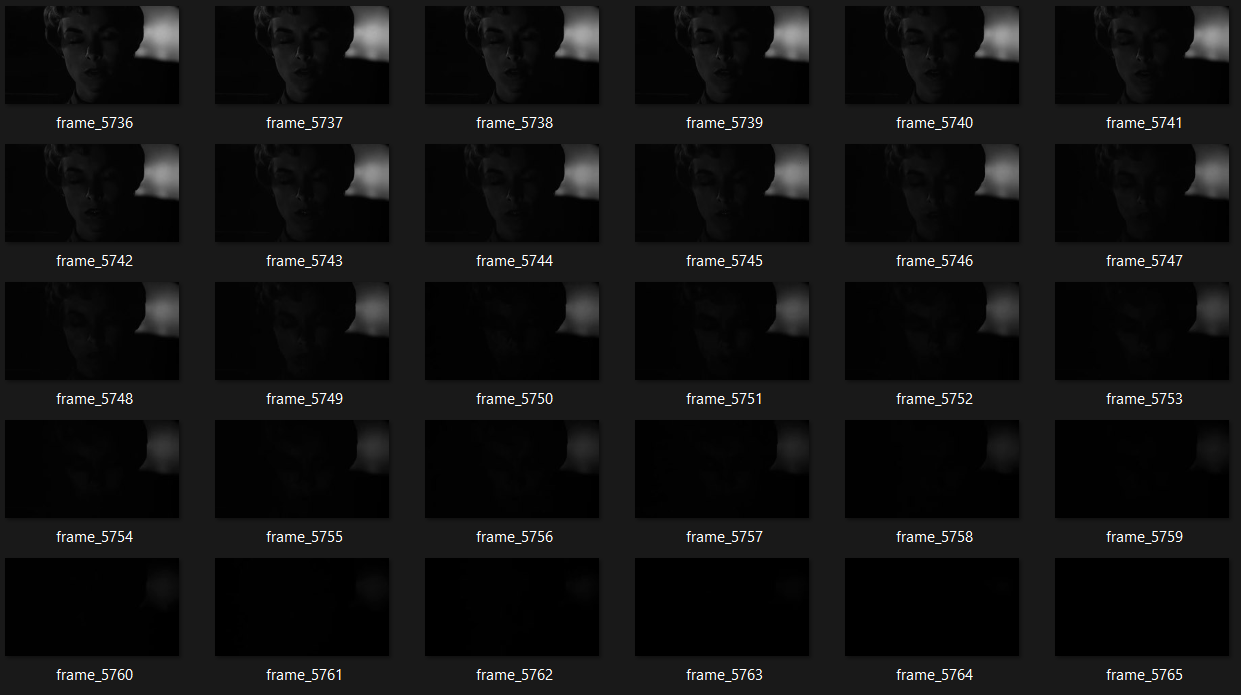
\includegraphics[width=\linewidth]{example_fade_out_transition.png}
			\caption{Example of a fade out transition}
			\label{fig:fade_out}
		\end{minipage}
		\hspace{0.05\linewidth}  % Space between the figures
		\begin{minipage}{0.45\linewidth}
			\centering
			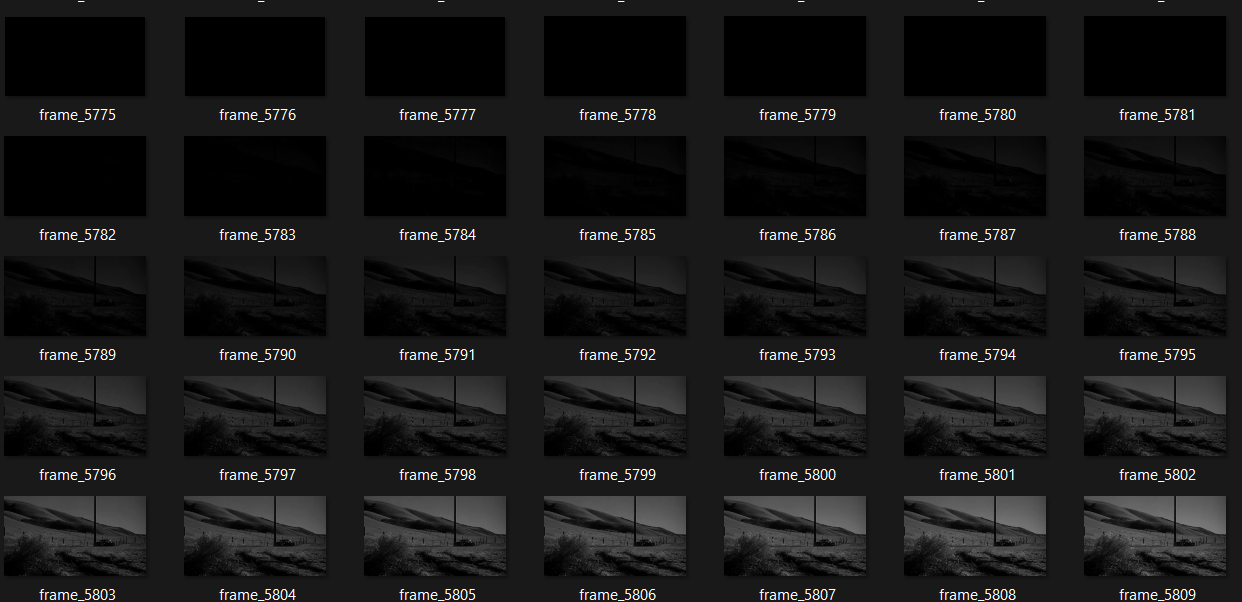
\includegraphics[width=\linewidth]{example_fade_in_transition.png}
			\caption{Example of fade in transition}
			\label{fig:fade_in}
		\end{minipage}
	\end{figure}
	
	\begin{figure}[h]
		\centering
		\begin{minipage}{0.45\linewidth}
			\centering
			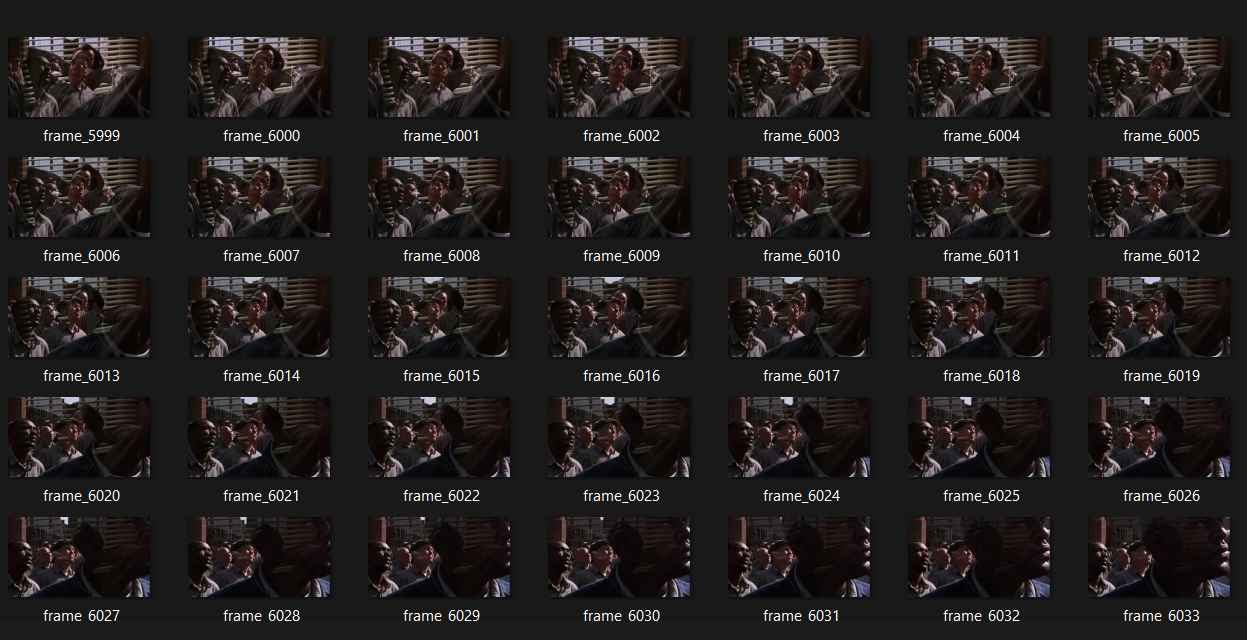
\includegraphics[width=\linewidth]{example_dissolve_transition.png}
			\caption{Example of a dissolve transition}
			\label{fig:dissolve}
		\end{minipage}
		\hspace{0.05\linewidth}  % Space between the figures
		\begin{minipage}{0.45\linewidth}
			\centering
			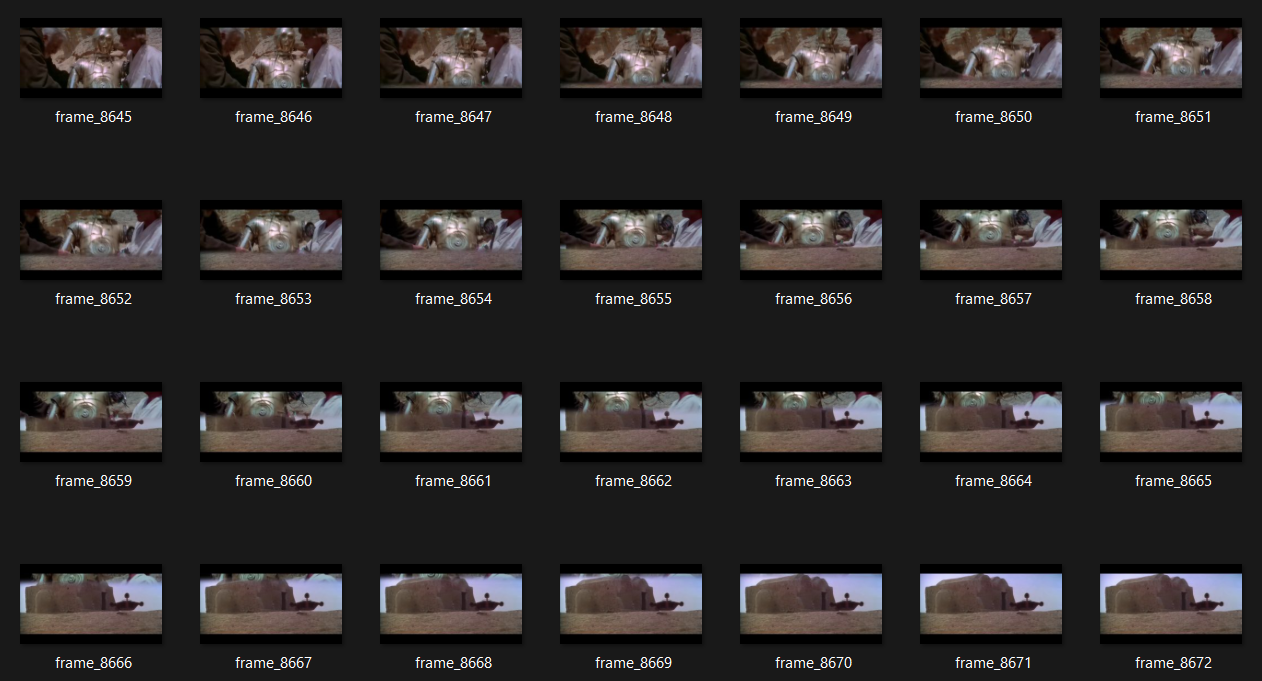
\includegraphics[width=\linewidth]{example_wipe_transition.png}
			\caption{Example of wipe transition}
			\label{fig:wipe}
		\end{minipage}
	\end{figure}
	
	
	\begin{algorithm}
		\caption{Shot Boundary Detection using SigLIP Features}
		\label{alg:shot-detection}
		\begin{algorithmic}[1]
			\Require Pre-trained model SigLIP, video frames $\{F_1, F_2, ..., F_N\}$, threshold $\tau$
			\Ensure Shot boundaries detected
			
			\For{$n = 1$ to $N-1$} \Comment{Iterate through video frames}
			\State $v_n \gets \text{ExtractFeatures}(F_n)$  \Comment{Extract feature vector for frame $n$}
			\State $v_{n+1} \gets \text{ExtractFeatures}(F_{n+1})$  \Comment{Extract feature vector for frame $n+1$}
			\State $\text{similarity} \gets \text{CosineSimilarity}(v_n, v_{n+1})$
			\If{$\text{similarity} < \tau$}
			\State \textbf{Mark} $F_n$ as a shot boundary
			\EndIf
			\EndFor
		\end{algorithmic}
	\end{algorithm}
	

	
	\begin{figure}[h]  % "h" places it approximately here
		\centering
		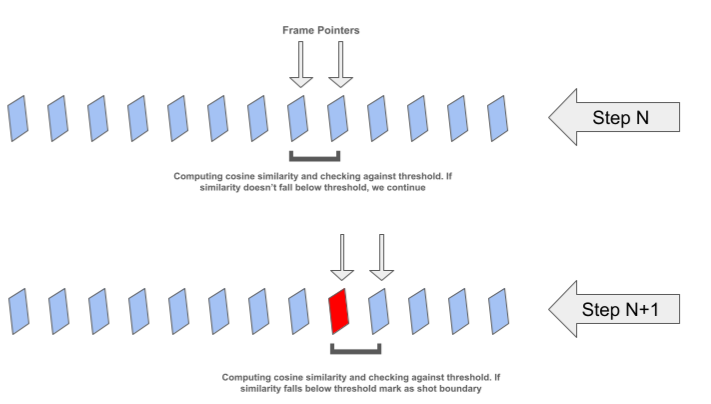
\includegraphics[width=\linewidth]{sbd_illustration.png}  % Adjust width as needed
		\caption{Illustration of Shot Boundary Detection with SigLIP and Cosine Similarity}
		\label{fig:sbd_illustration}
	\end{figure}
	
	
	\subsection{Key Shot Extraction or Key Frame Extraction (KSE or KFE)}
	
	According to Nyquist’s theorem \cite{adc}, to reconstruct an analog signal digitally, the digital system must capture the analog signal at twice the highest frequency component in the analog signal. In this instance the analog signal is the visible spectrum of light rays reflected from an object. \cite{fps} To capture the motion of an object we need to capture frames at one of the following frame rates per second : (1) 24 (2) 48 (3) 60. As a result in unit second we have a lot of similar frames that need to be processed. It seems redundant to look at near similar frames repeatedly. What if we could group frames based on their similarity? Key Shot Extraction allows us to represent a group of similar frames.
	

		
	
	Experimentation was done on one KSE methods. \cite{telnet} One existing method is by leveraging CNN models and image feature extraction models  like 3D CNNs, after we get the features we calculate the mean of the features extracted from the frames within a shot. Using this mean feature vector we use euclidean distance to find a frame that is closest to this mean feature vector. This is process illustrated in Algorithm~\ref{alg:rep-frame-selection}
	
\begin{algorithm}
	\caption{Representative Frame Selection using 3D CNN Features \cite{telnet}}
	\label{alg:rep-frame-selection}
	\begin{algorithmic}[1]
		\State \textbf{Input:} Video shot frames $\{F_1, F_2, ..., F_N\}$, pre-trained 3D CNN model
		\State \textbf{Output:} Representative frame $F_{\text{rep}}$
		
		\For{$n = 1$ to $N$} \Comment{Extract features for all frames}
		\State $v_n \gets \text{ExtractFeatures}(F_n)$ \Comment{Feature vector from 3D CNN}
		\EndFor
		
		\State $v_{\text{mean}} \gets \frac{1}{N} \sum_{n=1}^{N} v_n$ \Comment{Compute mean feature vector}
		
		\State $F_{\text{rep}} \gets F_1$  \Comment{Initialize representative frame}
		\State $d_{\text{min}} \gets \infty$ \Comment{Initialize minimum distance}
		
		\For{$n = 1$ to $N$} \Comment{Find closest frame to mean}
		\State $d \gets \text{EuclideanDistance}(v_n, v_{\text{mean}})$
		\If{$d < d_{\text{min}}$}
		\State $d_{\text{min}} \gets d$
		\State $F_{\text{rep}} \gets F_n$
		\EndIf
		\EndFor
		
		\State \Return $F_{\text{rep}}$
	\end{algorithmic}
\end{algorithm}
	\subsection{Video Classification}
	The final step in this pipeline is video classification, we feed the keyshots to the model to classify the shot into one of the following:(1) Fight (2) Rescue (3) Capture (4) Heist (5) Pursuit (6) Speed and (7) Pursuit. For this project we experiment with llava interleave \cite{llava} with a Qwen LLM backend. More details will be shown in the experimentation section.
	\section{Dataset}
	We craft a dataset to evaluate Shot Boundary Detection. Details for access to this dataset can be found under Appendix~\ref{app:sbd_dataset}. This dataset has been created with the movie "The Wild Bunch (1969)", we use 9 minutes of the film to evaluate the shot boundary. Additionally, we also create a dataset of the action forms present in the film to evaluate which approach would be suitable for video classification.
	\section{Experiments}
	To choose the best techniques for shot boundary detection, key shot extraction and video classification some experimentation was carried out. Most experiments were carried out on a NVIDIA TITAN RTX GPU with CUDA Version 12.3 and 24GB of GPU memory. The subsequent sections discuss the experiments performed.
	\subsection{Autoshot vs Cosine Similarity of SigLIP extracted features for Shot Boundary Detection}
	
	We test both the algorithms against the dataset dataset described in Appendix~\ref{app:sbd_dataset}. We run Autoshot and our algorithm against this dataset for evaluation. We generate the shots on the film "The Wild Bunch (1969)", the data generated from both the algorithms is described in Appendix~\ref{app:sbd_data_generated}.
	\subsection{Video Classification with Euclidean based Keyshots}
	
	We experiment zero shot video classification with two variants of the "llava-interleave-qwen" model (1) 0.5 billion parameter model and (2) 7 billion parameter model. We use the same prompt in both cases and try to annotate the keyshots extracted by  and evaluate them using cosine similarity loss as given by Equation~\eqref{eq:cosine_loss} where $a$ and $b$ is the feature vector of the labels for the ground truth dataset and zero-shot annotation done by LLaVA. Additionally, we fine tune the 0.5 billion parameter model using Quantized Low Rank Adaptation (QLoRA) method and compare the output of this model with the other two models.
	
	\begin{equation}
		\mathcal{L}_{\text{cosine}} = 1 - \frac{\mathbf{a} \cdot \mathbf{b}}{\|\mathbf{a}\| \|\mathbf{b}\|}
		\label{eq:cosine_loss}
	\end{equation}
	
	where:
	\begin{itemize}
		\item \( \mathcal{L}_{\text{cosine}} \) is the cosine similarity loss, which measures the dissimilarity between two vectors.
		\item \( \mathbf{a} \) is the first vector.
		\item \( \mathbf{b} \) is the second vector.
		\item \( \mathbf{a} \cdot \mathbf{b} \) is the dot product of vectors \( \mathbf{a} \) and \( \mathbf{b} \).
		\item \( \|\mathbf{a}\| \) is the Euclidean norm (magnitude) of vector \( \mathbf{a} \), calculated as \( \|\mathbf{a}\| = \sqrt{\sum_{i=1}^{n} a_i^2} \).
		\item \( \|\mathbf{b}\| \) is the Euclidean norm (magnitude) of vector \( \mathbf{b} \), calculated similarly.
		\item The formula calculates the cosine of the angle between vectors \( \mathbf{a} \) and \( \mathbf{b} \), and the loss is the complement of the cosine similarity, where a higher value indicates greater dissimilarity.
	\end{itemize}

	% Results and Discussion (New Page)
	\newpage
	\chapter{Results and Discussion}
	
\section{Autoshot vs Cosine Similarity of SigLIP extracted}

During our experiments we found that Autoshot was good at detecting cut transitions but not gradual transitions. Additionally, it is not robust to changes in lighting as shown in Figure~\ref{fig:autoshot_lighting_imapact}, where as our approach is robust to some degree of lighting changes as shown in Figure~\ref{fig:siglip_lighting_imapact}. Furthermore, we see that SigLIP outperforms Autoshot to detect fade transitions which is evident in figures~\ref{fig:auto_shot_fade_in},~\ref{fig:auto_shot_fade_out},~\ref{fig:siglip_fade_out} and ~\ref{fig:siglip_fade_in}. Table~\ref{tab:errors} shows how different thresholds of our algorithm has performed against Autoshot, the same can be seen in Figures~\ref{fig:sbd_start_error} and ~\ref{fig:sbd_end_error}. An ablation study of the thresholds shows that using a threshold 0.825 is the optimum threshold for shot boundary detection for the movie "The Wild Bunch(1969)". The optimum threshold may not be applicable for all movies, but what we can say for sure that an ideal threshold lies between 0.8 and 0.85, the same can be seen in Figure~\ref{fig:sbd_analysis_start} and Figure~\ref{fig:sbd_analysis_end}. Our approach to SBD fails to detect wipes and dissolves. We will discuss how improvements can be made to fix this deficiency in the Conclusion section.


\begin{figure}[h]  % "h" places it approximately here
	\centering
	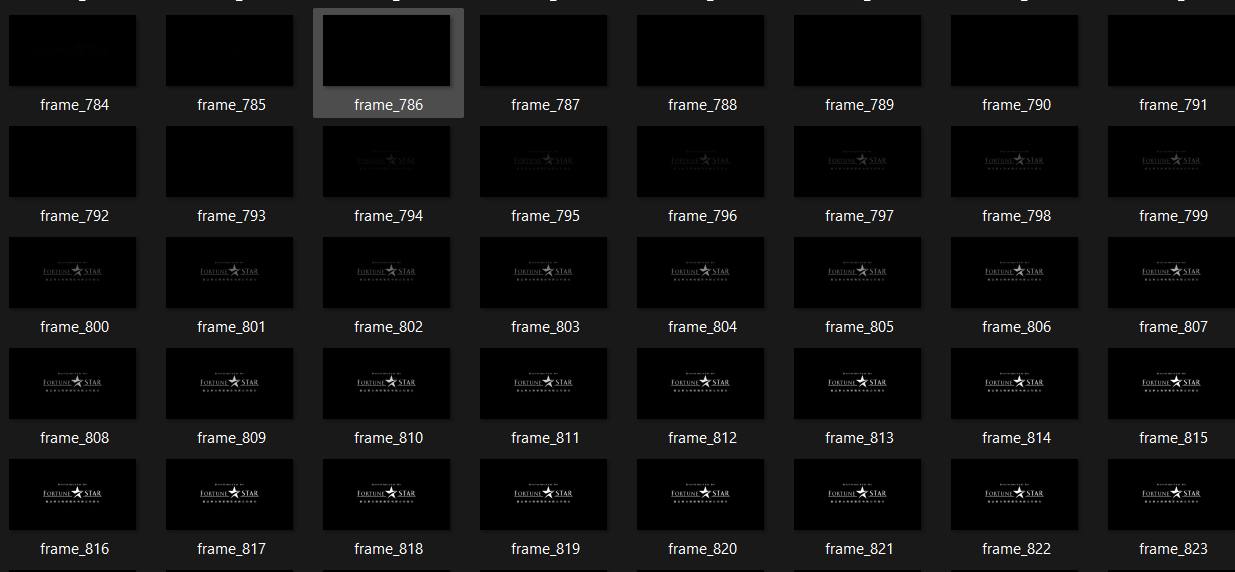
\includegraphics[width=\linewidth]{autoshot_fade_in.png}  % Adjust width as needed
	\caption{Shows that Autoshot fails to detect fade in}
	\label{fig:auto_shot_fade_in}
\end{figure}

\begin{figure}[h]  % "h" places it approximately here
	\centering
	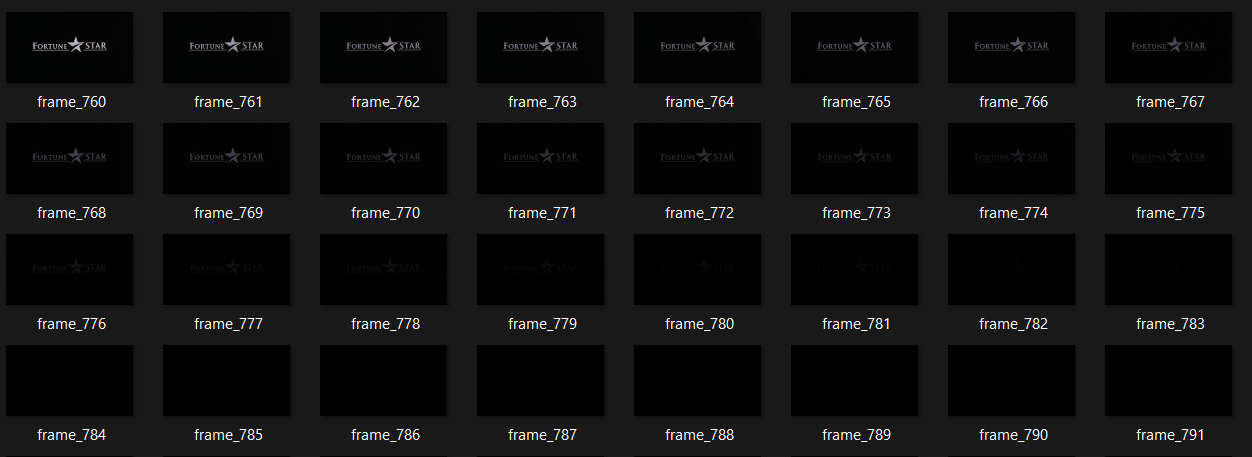
\includegraphics[width=\linewidth]{autoshot_fade_out.png}  % Adjust width as needed
	\caption{Shows that Autoshot fails to detect fade out}
	\label{fig:auto_shot_fade_out}
\end{figure}


\begin{figure}[h]  % "h" places it approximately here
	\centering
	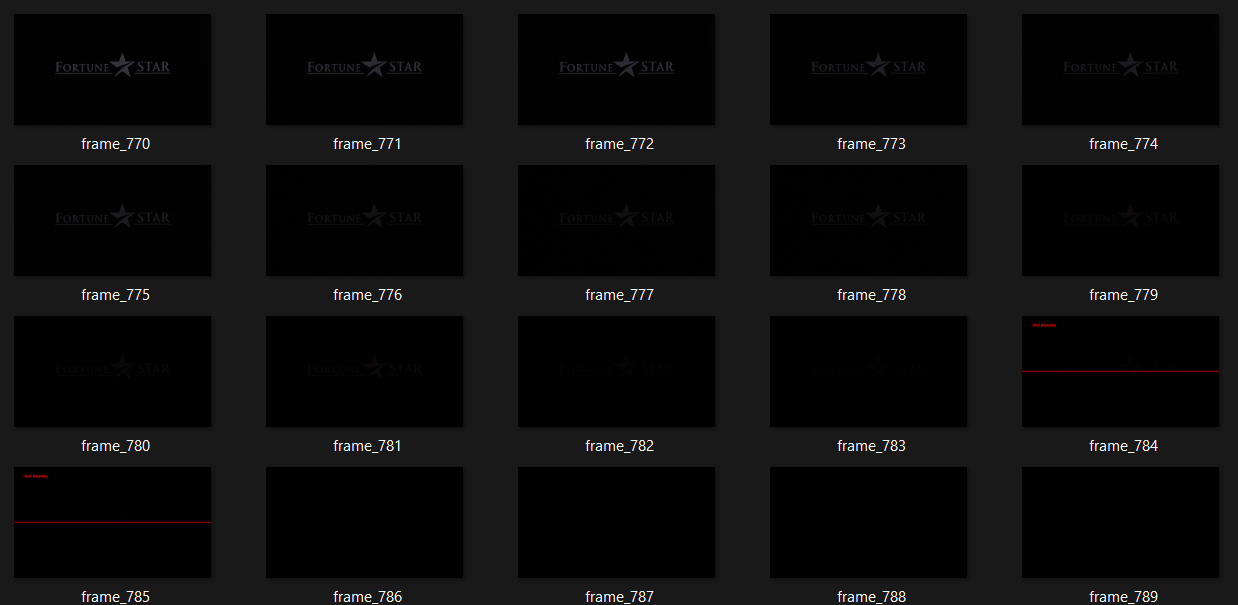
\includegraphics[width=\linewidth]{fade_out.png}  % Adjust width as needed
	\caption{Shows that ability of SigLIP to detect fade out transitions}
	\label{fig:siglip_fade_out}
\end{figure}

\begin{figure}[h]  % "h" places it approximately here
	\centering
	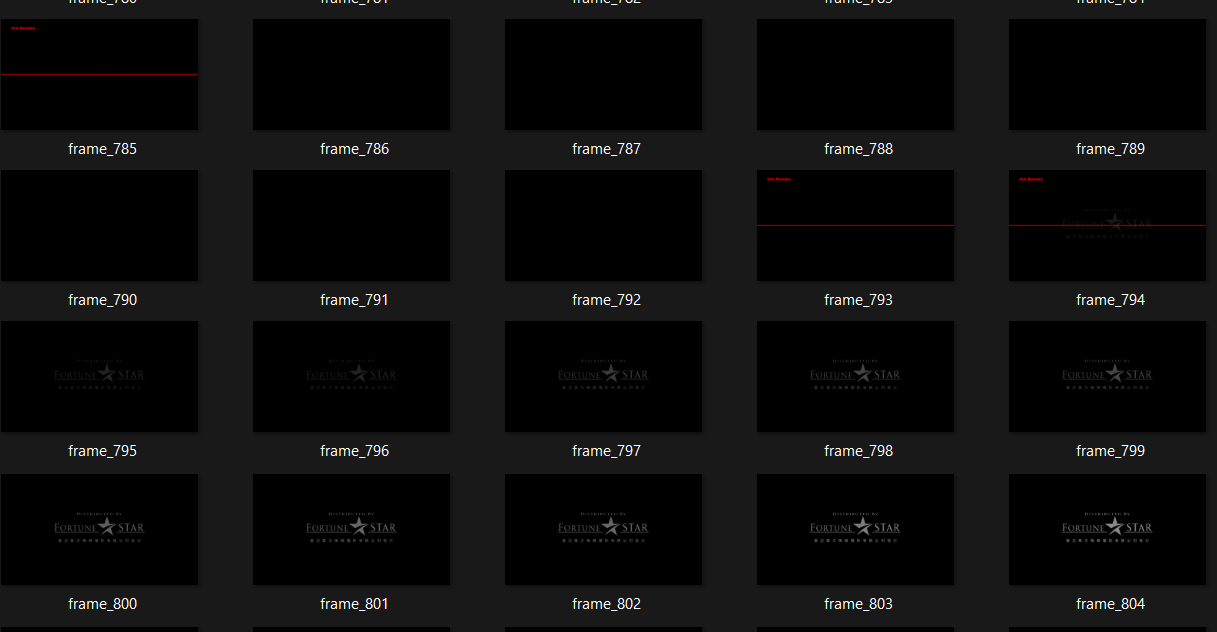
\includegraphics[width=\linewidth]{siglip_fade_in_transition.png}  % Adjust width as needed
	\caption{Shows that ability of SigLIP to detect fade in transitions}
	\label{fig:siglip_fade_in}
\end{figure}

\begin{table}[h]
	\centering
	\resizebox{\textwidth}{!}{ % Resize table to fit within text width
		\begin{tabular}{lcccc}
			\toprule
			\textbf{Thresholds \& Algorithm} & \textbf{Start Mean Error} & \textbf{Start Std Error} & \textbf{End Mean Error } & \textbf{End Std Error} \\
			\midrule
			0.7       & 355.1162  & 317.1224  & 364.8854  & 328.0517  \\
			0.75      & 110.2121  & 73.8650   & 111.2194  & 73.3501   \\
			0.8       & 31.7705   & 30.4009   & 32.1423   & 30.3124   \\
			0.825     & 14.0106   & 8.9510    & 14.0325   & 8.8707    \\
			0.85      & 32.7118   & 14.3814   & 33.1615   & 14.4939   \\
			0.9       & 96.8780   & 39.7198   & 97.7498   & 39.0056   \\
			Autoshot  & 27.5037   & 14.1594   & 27.8982   & 14.3291   \\
			\bottomrule
		\end{tabular}
	}
	\caption{Performance summary of various SigLIP thresholds and the Autoshot algorithm against the dataset in Appendix~\ref{app:sbd_dataset}.}
	\label{tab:errors}
\end{table}

\begin{equation}
	\text{SME} = \frac{1}{N} \sum_{i=1}^{N} \left| \text{Predicted\_Start}_i - \text{Actual\_Start}_i \right|
	\label{eq:sme}
\end{equation}

where:
\begin{itemize}
	\item \( SME \) is the Start Mean Error.
	\item \( N \) is the total number of samples.
	\item \( \text{Predicted\_Start}_i \) is the predicted start value for the \( i \)-th sample.
	\item \( \text{Actual\_Start}_i \) is the actual start value for the \( i \)-th sample.
	\item \( |\cdot| \) denotes the absolute value operation.
\end{itemize}
\begin{equation}
	\text{EME} = \frac{1}{N} \sum_{i=1}^{N} \left| \text{Predicted\_End}_i - \text{Actual\_End}_i \right|
	\label{eq:eme}
\end{equation}

where:
\begin{itemize}
	\item \( EME \) is the End Mean Error.
	\item \( N \) is the total number of samples.
	\item \( \text{Predicted\_End}_i \) is the predicted end value for the \( i \)-th sample.
	\item \( \text{Actual\_End}_i \) is the actual end value for the \( i \)-th sample.
	\item \( |\cdot| \) denotes the absolute value operation.
\end{itemize}

\begin{equation}
	\text{Start Std Error} = \sqrt{\frac{1}{N} \sum_{i=1}^{N} \left( y_i - \mu_y \right)^2}
	\label{eq:start_std_error}
\end{equation}

where:
\begin{itemize}
	\item \(\text{Start Std Error}\) represents the standard deviation of the absolute start errors.
	\item \( N \) is the total number of samples.
	\item \( y_i \) is the absolute error for the \( i \)-th sample, defined as:
	
	\[
	y_i = |\text{Predicted\_Start}_i - \text{Actual\_Start}_i|
	\]
	
	\item \( \mu_y \) is the mean absolute error, given by:
	
	\[
	\mu_y = \frac{1}{N} \sum_{i=1}^{N} y_i
	\]
	
	\item \( (\cdot)^2 \) denotes squaring the term inside the parentheses.
	\item \( \sqrt{\cdot} \) represents the square root operation.
\end{itemize}
\begin{equation}
	\text{End Std Error} = \sqrt{\frac{1}{N} \sum_{i=1}^{N} \left( y_i - \mu_y \right)^2}
	\label{eq:end_std_error}
\end{equation}

where:
\begin{itemize}
	\item \(\text{End Std Error}\) represents the standard deviation of the absolute end errors.
	\item \( N \) is the total number of samples.
	\item \( y_i \) is the absolute error for the \( i \)-th sample, defined as:
	
	\[
	y_i = |\text{Predicted\_End}_i - \text{Actual\_End}_i|
	\]
	
	\item \( \mu_y \) is the mean absolute error, given by:
	
	\[
	\mu_y = \frac{1}{N} \sum_{i=1}^{N} y_i
	\]
	
	\item \( (\cdot)^2 \) denotes squaring the term inside the parentheses.
	\item \( \sqrt{\cdot} \) represents the square root operation.
\end{itemize}
\begin{equation}
	\text{End Std Error} = \sqrt{\frac{1}{N} \sum_{i=1}^{N} \left( y_i - \mu_y \right)^2}
	\label{eq:end_std_error}
\end{equation}

where:
\begin{itemize}
	\item \(\text{End Std Error}\) represents the standard deviation of the absolute end errors.
	\item \( N \) is the total number of samples.
	\item \( y_i \) is the absolute error for the \( i \)-th sample, defined as:
	
	\[
	y_i = |\text{Predicted\_End}_i - \text{Actual\_End}_i|
	\]
	
	\item \( \mu_y \) is the mean absolute error, given by:
	
	\[
	\mu_y = \frac{1}{N} \sum_{i=1}^{N} y_i
	\]
	
	\item \( (\cdot)^2 \) denotes squaring the term inside the parentheses.
	\item \( \sqrt{\cdot} \) represents the square root operation.
\end{itemize}


\begin{equation}
	\text{End Std Error} = \sqrt{\frac{1}{N} \sum_{i=1}^{N} \left( y_i - \mu_y \right)^2}
	\label{eq:end_std_error}
\end{equation}

where:
\begin{itemize}
	\item \(\text{End Std Error}\) represents the standard deviation of the absolute end errors.
	\item \( N \) is the total number of samples.
	\item \( y_i \) is the absolute error for the \( i \)-th sample, defined as:
	
	\[
	y_i = |\text{Predicted\_End}_i - \text{Actual\_End}_i|
	\]
	
	\item \( \mu_y \) is the mean absolute error, given by:
	
	\[
	\mu_y = \frac{1}{N} \sum_{i=1}^{N} y_i
	\]
	
	\item \( (\cdot)^2 \) denotes squaring the term inside the parentheses.
	\item \( \sqrt{\cdot} \) represents the square root operation.
\end{itemize}

\begin{figure}[h]  % "h" places it approximately here
	\centering
	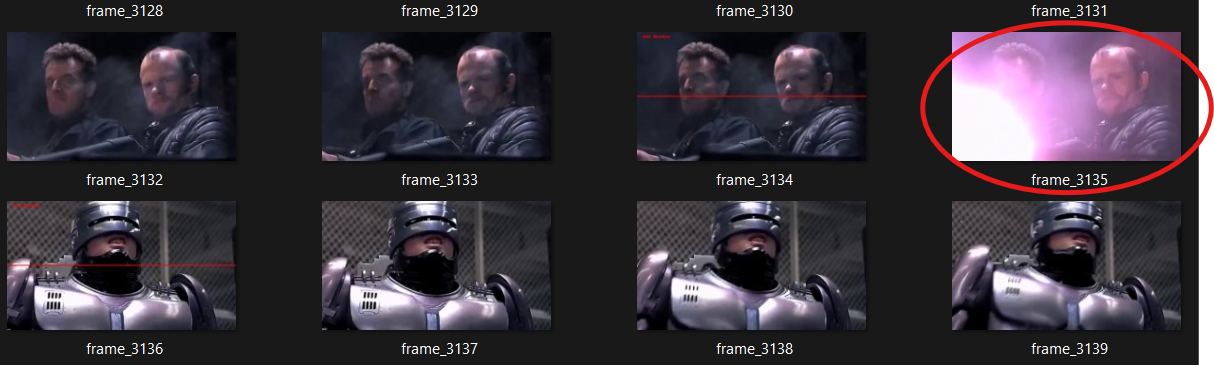
\includegraphics[width=\linewidth]{autoshot_lighting_impact.png}  % Adjust width as needed
	\caption{Shows that Autoshot cuts shot boundaries when the lighting changes}
	\label{fig:autoshot_lighting_imapact}
\end{figure}
\begin{figure}[h]  % "h" places it approximately here
	\centering
	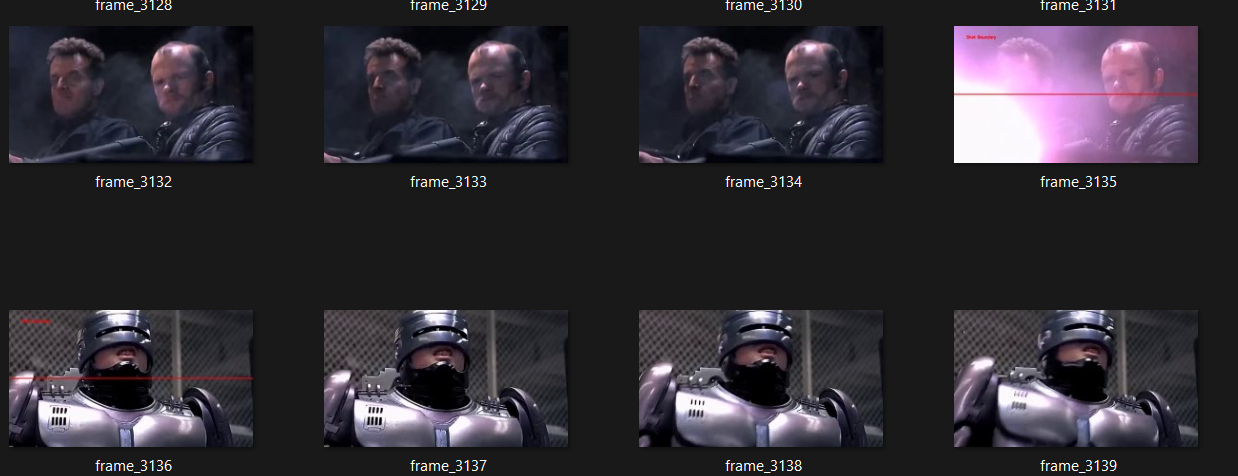
\includegraphics[width=\linewidth]{siglip_ligting_impact.png}  % Adjust width as needed
	\caption{Shows SigLIPs Robustness to lighting changes}
	\label{fig:siglip_lighting_imapact}
\end{figure}
		\begin{figure}[h]  % "h" places it approximately here
		\centering
		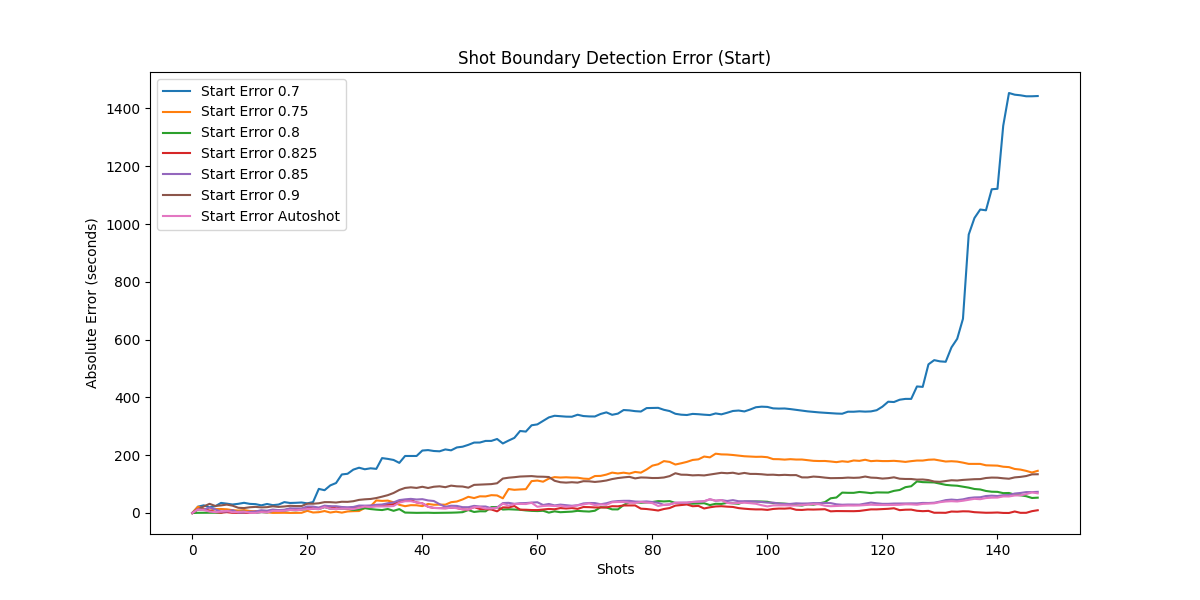
\includegraphics[width=\linewidth]{sbd_start_error.png}  % Adjust width as needed
		\caption{Shot Boundary Start Error Results for 149 shots}
		\label{fig:sbd_start_error}
	\end{figure}
	
	\begin{figure}[h]  % "h" places it approximately here
		\centering
		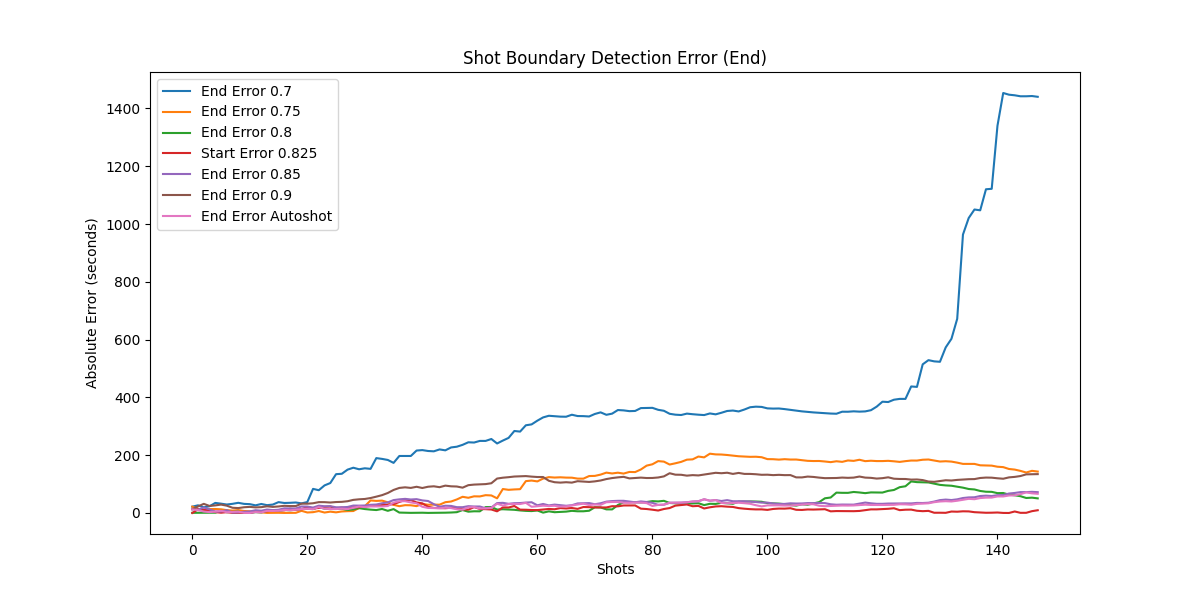
\includegraphics[width=\linewidth]{sbd_end_error.png}  % Adjust width as needed
		\caption{Shot Boundary End Error Results for 149 shots}
		\label{fig:sbd_end_error}
	\end{figure}
	\begin{figure}[h]  % "h" places it approximately here
		\centering
		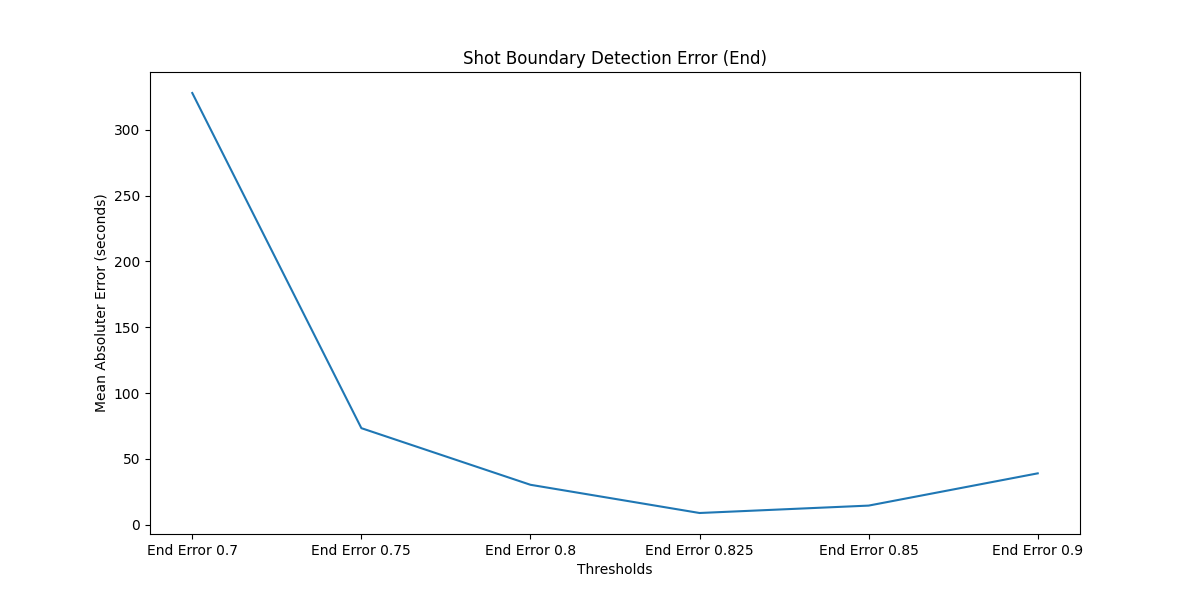
\includegraphics[width=\linewidth]{analysis_5.png}  % Adjust width as needed
		\caption{Illustration of effect of threshold on accuracy of shot boundary clip end points}
		\label{fig:sbd_analysis_end}
	\end{figure}
	\begin{figure}[h]  % "h" places it approximately here
		\centering
		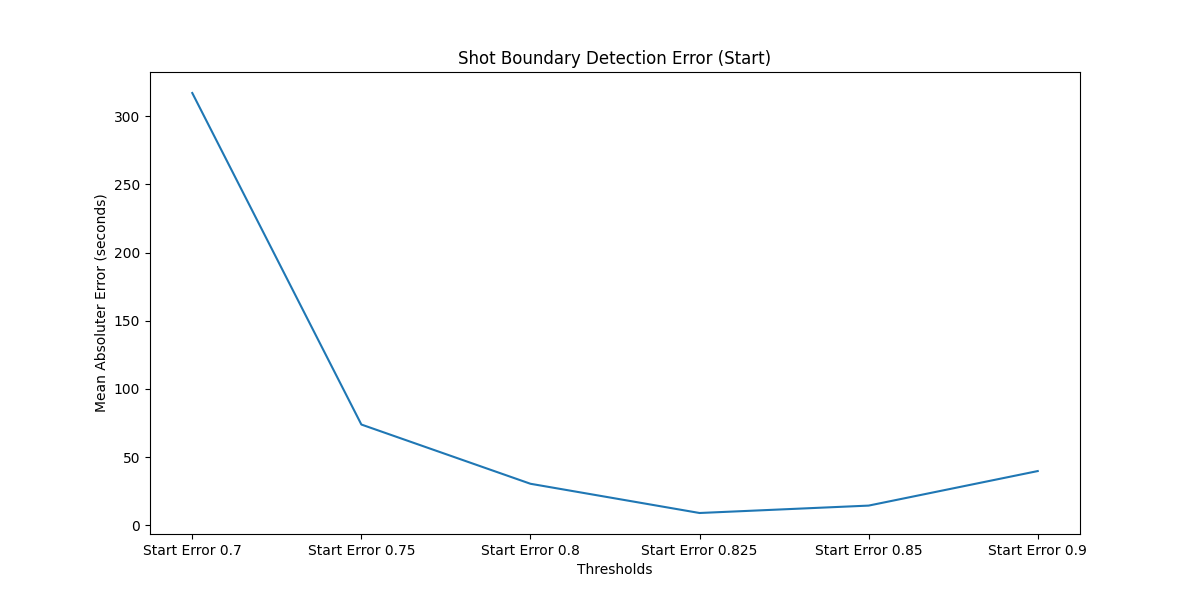
\includegraphics[width=\linewidth]{analysis_6.png}  % Adjust width as needed
		\caption{Illustration of effect of threshold on accuracy of shot boundary clip start points}
		\label{fig:sbd_analysis_start}
	\end{figure}
	% Conclusion (New Page)
	\section{Video Classification with Euclidean based Keyshot Extraction}
	
	In our experiment, we try to evaluate whether Euclidean based keyshot extraction. The resulting data for zero shot video classification with Euclidean based can be seen under Appendix~\ref{app:zero_shot_euclidean_classification}. From the results we can see that LLaVA with 0.5 billion parameters doesn't follow the instructions while the 7 billion parameter variant does. The performance of the two models is shown in Figure~\ref{fig:loss_analysis}. From this experiment we found that a window size 5 is best suited for inference given the computing resource constraint, beyond that you would run out of memory when using the GPU. Additionally, we can see that the 7 billion parameter model produces near similar embeddings we need for annotating films. Furthermore, we try to fine-tune both models, fine-tuning the 7 billion parameter is impossible with the current compute, but it is possible 
	to train the 0.5 billion parameter since it consumes less GPU memory during training . The same can be estimated using the formula given in Equation~\ref{eq:memory_calculation} which is used in \cite{calculator} to estimate memory consumption. Figure~\ref{fig:loss_analysis} summarizes the performance these models on euclidean based keyshot extraction. From Table~\ref{tab:cosine_loss} we can see that zero shot prompting produces vectors some degree of dissimilarity, whereas Supervised fine-tuning produces similar vectors with some intermittent inaccuracies.
	
	
	\begin{table}[h]
		\centering
		\begin{tabular}{lcc}
			\toprule
			\textbf{Model} & \textbf{Mean Cosine Loss} & \textbf{Standard Deviation of Cosine Loss} \\
			\midrule
			llava 0.5B parameter model & 0.3952 & 0.0806 \\
			llava 7B parameter model & 0.3459 & 0.0303 \\
			sft trained llava 0.5B parameter & 0.0859 & 0.0907 \\
			\bottomrule
		\end{tabular}
		\caption{Mean and Standard Deviation of Cosine Loss for Different Models}
		\label{tab:cosine_loss}
	\end{table}
	
	
	\begin{figure}[h]  % "h" places it approximately here
		\centering
		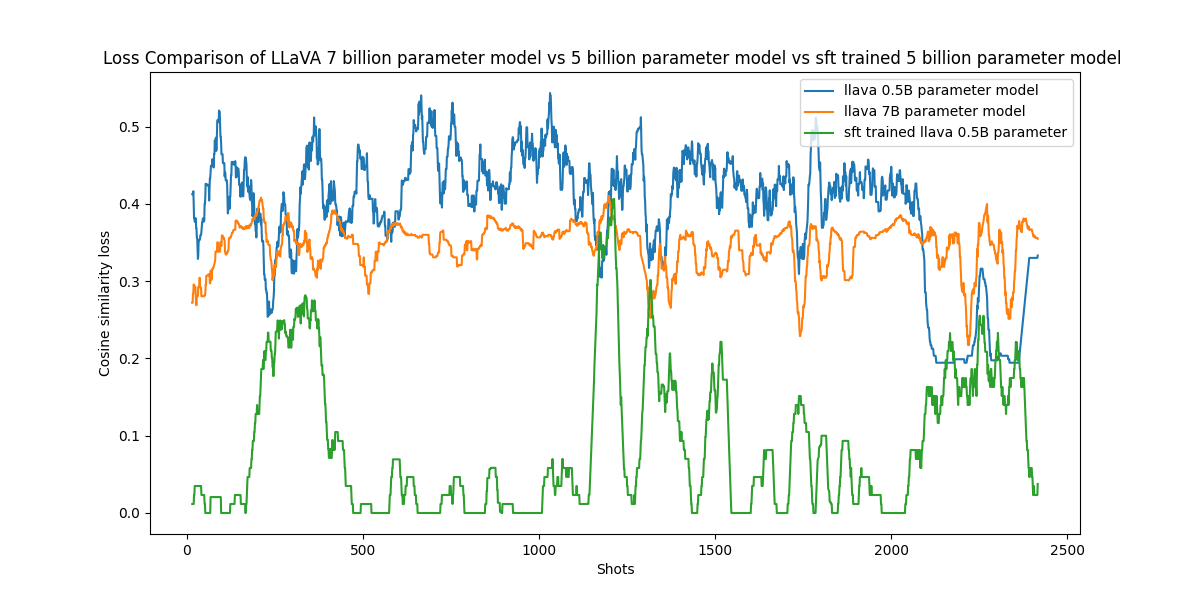
\includegraphics[width=\linewidth]{loss_analysis.png}  % Adjust width as needed
		\caption{Shows loss analysis of various models we experimented against euclidean base key shot extraction}
		\label{fig:loss_analysis}
	\end{figure}
	
	\begin{equation}
		\label{eq:memory_calculation}
		\text{Memory (GB)} = \frac{\text{Parameters (billions)} \times \text{BytesPerParameter} \times 6}{1024^3}
	\end{equation}
	
	\newpage
	\chapter{Conclusion}
	From the project we have obtained a way to extract shots that are relevant to the story unit. We also find that additional work needs to be done to detect dissolve and wipe transitions which are gradual transitions i.e. transitions which happens over several frames. The shortcoming with the approach used in the project is that we are accounting for changes in 2 frames we need to account for changes in several frames, we need to use a window and calculate how several frames change with respect to the first. This could potentially even eliminate the need for keyshot extraction, since you are already grouping frames with respect to the first frame in a given window. Keeping this window size dynamic i.e. cutting the window only when the similarities of the frame falls below a certain threshold. This could help group relevant frames and help provide granular details for the film. However, based on the threshold you might lose the relevant context i.e higher granularity will lead loss in context that might be relevant for the next shot.
	
	From our project we can see we can get more gains in annotating films by supervised fine-tuning, additionally, the inference time is greatly reduced. However, the model seems to be good at only detecting "No Action Found" and "Fight" scenes. This is due to the imbalanced dataset that we have. We need more data on the other action scenarios as well.
	
	To summarise the improvements that needs to be done (1) increase the window size for shot detection and (2) collect more data on the other action scenarios.
	 
	% References (IEEE Format, New Page)
	\newpage
	\begin{thebibliography}{99}
		\bibitem{tico-romao-2024} 
		T. Romao, "How to analyze action in film," Action-Cinema.com, Jan. 13, 2024. [Online]. Available: \url{https://action-cinema.com/?p=1184}.
		\bibitem{chris-baldwin} C. G. Baldick, “The Concise Oxford dictionary of literary terms,” Choice Reviews Online, vol. 28, no. 09, pp. 28–4843, May 1991, doi: 10.5860/choice.28-4843.
		\bibitem{h_w-chen}H.-W. Chen, J.-H. Kuo, W.-T. Chu, and J.-L. Wu, “Action movies segmentation and summarization based on tempo analysis,” MIR ’04: Proceedings of the 6th ACM SIGMM International Workshop on Multimedia Information Retrieval, pp. 251–258, Oct. 2004, doi: 10.1145/1026711.1026752.
		\bibitem{zhang}B. Yu, W.-Y. Ma, K. Nahrstedt, and H.-J. Zhang, “Video summarization based on user log enhanced link analysis,” ACM MM ’03, pp. 382–391, Nov. 2003, doi: 10.1145/957013.957095.
		\bibitem{i-laptev}I. Laptev, M. Marszalek, C. Schmid, and B. Rozenfeld, “Learning realistic human actions from movies,” 2009 IEEE Conference on Computer Vision and Pattern Recognition, Jun. 2008, doi: 10.1109/cvpr.2008.4587756.
		\bibitem{gaidon}A. Gaidon, M. Marszalek, and C. Schmid, “Mining visual actions from movies,” British Machine Vision Conference, British Machine Vision Association, Sep 2009, Londres, United Kingdom, p. 125.1-125.11, Jan. 2009, doi: 10.5244/c.23.125.
		\bibitem{kulkarni}K. Kulkarni, G. Evangelidis, J. Cech, and R. Horaud, “Continuous action recognition based on sequence alignment,” International Journal of Computer Vision, vol. 112, no. 1, pp. 90–114, Sep. 2014, doi: 10.1007/s11263-014-0758-9.
		\bibitem{c_f_chen}C.-F. Chen et al., “Deep analysis of CNN-based spatio-temporal representations for action recognition,” arXiv (Cornell University), Jan. 2020, doi: 10.48550/arxiv.2010.11757.
		\bibitem{g-yao}G. Yao, T. Lei, and J. Zhong, “A review of Convolutional-Neural-Network-based action recognition,” Pattern Recognition Letters, vol. 118, pp. 14–22, May 2018, doi: 10.1016/j.patrec.2018.05.018.
		\bibitem{manakitsa}N. Manakitsa, G. S. Maraslidis, L. Moysis, and G. F. Fragulis, “A review of machine learning and deep learning for object detection, semantic segmentation, and human action recognition in machine and robotic vision,” Technologies, vol. 12, no. 2, p. 15, Jan. 2024, doi: 10.3390/technologies12020015.
		\bibitem{llms}H. Qu, Y. Cai, and J. Liu, “LLMs are Good Action Recognizers,” 2022 IEEE/CVF Conference on Computer Vision and Pattern Recognition (CVPR), vol. 33, pp. 18395–18406, Jun. 2024, doi: 10.1109/cvpr52733.2024.01741.
		\bibitem{sbd}B. A. Halim and T. Faiza, “Shot Boundary Detection: Fundamental Concepts and Survey.,” Conference on Innovative Trends in Computer Science, pp. 34–40, Jan. 2019, [Online]. Available: http://ceur-ws.org/Vol-2589/Paper6.pdf
		\bibitem{siglip}X. Zhai, B. Mustafa, A. Kolesnikov, and L. Beyer, “Sigmoid loss for language image Pre-Training,” arXiv (Cornell University), Jan. 2023, doi: 10.48550/arxiv.2303.15343.
		\bibitem{adc}H. Austerlitz, “Analog/Digital conversions,” in Elsevier eBooks, 2003, pp. 51–77. doi: 10.1016/b978-012068377-2/50004-8.
		\bibitem{fps} L. M. Wilcox, R. S. Allison, J. Helliker, B. Dunk, and R. C. Anthony, “Evidence that Viewers Prefer Higher Frame-Rate Film,” ACM Transactions on Applied Perception, vol. 12, no. 4, pp. 1–12, Sep. 2015, doi: 10.1145/2810039.
		\bibitem{telnet}S.-M. Tseng, Z.-T. Yeh, C.-Y. Wu, J.-B. Chang, and M. Norouzi, “Video scene detection using transformer Encoding Linker Network (TELNet),” Sensors, vol. 23, no. 16, p. 7050, Aug. 2023, doi: 10.3390/s23167050.
		\bibitem{llava} H. Liu, C. Li, Q. Wu, and Y. J. Lee, “Visual instruction tuning,” arXiv (Cornell University), Jan. 2023, doi: 10.48550/arxiv.2304.08485.
		\bibitem{calculator} “LLM GPU Memory Calculator — Twinko AI,” Twinko AI. https://www.twinko.ai/app/llm-gpu-memory-calculator
	\end{thebibliography}
	
	% Appendices (New Page)
	\newpage
	\appendix
	\addcontentsline{toc}{chapter}{Appendices}
	\renewcommand{\thechapter}{\Alph{chapter}} 
	\chapter{Dataset for Shot Boundary Detection Evaluation} \label{app:sbd_dataset}
	\textbf{Dataset used for evaluation: }\href{https://drive.google.com/file/d/1WiPqupmqC01gvXg4dfgqHFHf6UBJJ1yL/view?usp=drive_link} {Evaluation Data For Shot Boundary}
	\chapter{Dataset for Various Action forms in the movie} \label{app:action_forms_dataset}
	\textbf{Action Profiles:}\href{https://drive.google.com/drive/folders/1APxsIVRthZuePmZua_LhvEbFcj9B0X0M?usp=drive_link}{Here}\\
	\textbf{Movies}:\href{https://drive.google.com/drive/folders/1OoYPjnf8rtZ3b8pJ0KLmMzW3GLqD5o5r?usp=drive_link}{Here}
	\chapter{Annotated Movie Dataset} \label {app:movie_dataset}
	\textbf{Annotated Movied Dataset used as ground truth for training and evaluation for video classification:}\href{https://drive.google.com/file/d/1dvnYdUYhl6zQzJggLgC5r36W0nDtqqzX/view?usp=drive_link}{Here}
	\chapter{Code for Data Preparation} \label{app:data_prep}
	\begin{lstlisting}[language=Python, caption={Video DataSet Preparator Python Code}]
		import os
import pandas as pd
import argparse
import ffmpeg
from PIL import Image
from tqdm import tqdm
import numpy as np
import json
import cv2

def extract_frame(video_path, frame_number):
    """
    Extracts a specific frame from a video given its frame number.
    
    :param video_path: Path to the video file.
    :param frame_number: Frame number to extract.
    :return: PIL Image of the extracted frame, or None if failed.
    """
    cap = cv2.VideoCapture(video_path)
    cap.set(cv2.CAP_PROP_POS_FRAMES, frame_number)  # Move to the desired frame
    
    ret, frame = cap.read()  # Read the frame
    cap.release()
    
    if ret:
        frame = cv2.cvtColor(frame, cv2.COLOR_BGR2RGB)  # Convert OpenCV BGR to RGB
        return Image.fromarray(frame)
    else:
        print(f"Error: Could not extract frame {frame_number}")
        return None

def load_from_json(json_file):
    """
    Loads a JSON file containing a list of sets (stored as lists).
    
    :param json_file: Path to the JSON file.
    :return: List of sets.
    """
    data = None
    with open(json_file, "r") as file:
        data = json.load(file)
        
    return data

def write_data_incrementally_to_json(data_iterable, filename="processed_data_1.json"):
    with open(filename, 'w') as f:
        f.write('[\n')  # Start the JSON array
        first = True
        for data_dict in tqdm(data_iterable,desc="Writing Data to File"):
            if not first:
                f.write(',\n')  # Add a comma between JSON objects
            json.dump(data_dict, f)
            first = False
        f.write('\n]')  # End the JSON array
        
def extract_frames_to_pil(video_path, start_frame, end_frame):
    probe = ffmpeg.probe(video_path)
    fps = eval(next(stream for stream in probe["streams"] if stream["codec_type"] == "video")["r_frame_rate"])
    width = int(next(stream for stream in probe["streams"] if stream["codec_type"] == "video")["width"])
    height = int(next(stream for stream in probe["streams"] if stream["codec_type"] == "video")["height"])
    start_time = start_frame / fps
    end_time = end_frame / fps
    out, _ = (
        ffmpeg
        .input(video_path, ss=start_time, to=end_time)  # Trim video
        .output("pipe:", format="rawvideo", pix_fmt="rgb24")  # Output raw RGB frames
        .run(capture_stdout=True, capture_stderr=True)  # Capture in memory
    )
    frame_size = width * height * 3
    frames = [
        Image.fromarray(np.frombuffer(out[i:i+frame_size], np.uint8).reshape((height, width, 3)), 'RGB')
        for i in range(0, len(out), frame_size)
    ]
    return frames
    
def process_data(video_path,data_file,shots_file,window=10,user_prompt="What is this?"):
    data_file_df = pd.read_csv(data_file)
    shots_file_df = pd.read_csv(shots_file)
    new_df = pd.concat([data_file_df,shots_file_df],axis=1)
    new_df["Action Formatted"] = new_df["Action"].fillna("No Action Found")
    os.makedirs("/storage/alton/keyshot_frames",exist_ok=True)
    frame_number = 0
    for index, row in tqdm(new_df.iterrows(),desc="Creating Data Set"):
        shot= row["Shot"]
        start =  0 if (shot-window) < 0 else (shot-window)
        end = shot+window
        frames = extract_frames_to_pil(video_path,start,end)
        toks = "<image>" * (len(frames))
        prompt = "<|im_start|>user"+ toks + f"\n{user_prompt}<|im_end|><|im_start|>assistant "+row["Action Formatted"]+ "<|im_end|>"
        image_paths = []
        for frame in frames:
            frame.save(f"/storage/alton/keyshot_frames/frame_{frame_number}.jpg")
            image_paths.append(f"/storage/alton/keyshot_frames/frame_{frame_number}.jpg")
            frame_number = frame_number + 1
        data_dict = dict()
        data_dict["prompt"] = prompt
        data_dict["frames"] = image_paths
        yield data_dict

def process_data_alternative(video_path,data_file,shots_file,user_prompt="What is this?"):
    data_file_df = pd.read_csv(data_file)
    key_shots = load_from_json(shots_file)
    data_file_df["Action Formatted"] = data_file_df["Action"].fillna("No Action Found")
    os.makedirs("/storage/alton/keyshot_frames_1",exist_ok=True)
    frame_number = 0
    for index, row in tqdm(data_file_df.iterrows(),desc="Creating Data Set"):
        image_paths = []
        key_shot_entry = key_shots[index]
        frames = []
        for entry in key_shot_entry:
            frames.append(extract_frame(video_path,entry))
        for frame in frames:
            frame.save(f"/storage/alton/keyshot_frames_1/frame_{frame_number}.jpg")
            image_paths.append(f"/storage/alton/keyshot_frames_1/frame_{frame_number}.jpg")
            frame_number = frame_number + 1
        toks = "<image>" * (len(frames))
        prompt = "<|im_start|>user"+ toks + f"\n{user_prompt}<|im_end|><|im_start|>assistant "+row["Action Formatted"]+ "<|im_end|>"
        data_dict = dict()
        data_dict["prompt"] = prompt
        data_dict["frames"] = image_paths
        yield data_dict
    
    
if __name__=="__main__":
    parser = argparse.ArgumentParser(description="Video DataSet Preparator")
    parser.add_argument('--video', type=str, help="Video path")
    parser.add_argument('--data', type=str, help="CSV data path")
    parser.add_argument('--shots',type=str, help="Shots CSV data path")
    parser.add_argument('--window',type=int, help="Number of frames you wanna annotate")
    parser.add_argument("--alternative", action="store_true", 
                    help="Use the alternative method for keyshots")
    args = parser.parse_args()
    video_path = args.video
    data_path = args.data
    shots_path = args.shots
    window = args.window
    prompt = """
    Classify the given video into the following actions:
    1. Rescue
    2. Escape 
    3. Capture 
    4. Heist
    5. Fight
    6. Pursuit
    7. None of the Above - For scenes that do not fall into any of the aforementioned categories.
    Your Reply can include multiple categories if possible. For example, a scene can have Rescue and Escape.
    """
    if not args.alternative:
        write_data_incrementally_to_json(process_data(video_path,data_path,shots_path,window,prompt))
    else:
        write_data_incrementally_to_json(process_data_alternative(video_path,data_path,shots_path,prompt))
    
    
    
	\end{lstlisting}
	\chapter{Code for Shot Boundary Detection} \label{app:sbd_code}
	
\begin{lstlisting}[language=Python,caption={Shot Boundary Detection Code}]
	from transformers import AutoProcessor, SiglipVisionModel
	import torch
	import argparse
	import cv2
	from PIL import Image
	import itertools
	from itertools import islice
	import os
	import csv
	import time
	from tqdm import tqdm
	import pandas as pd
	import ffmpeg
	
	
	device = "cuda" if torch.cuda.is_available() else "cpu"
	
	def video_to_pil_frames(video_path):
		print(f"Fetching Frames: {video_path}")
		video = cv2.VideoCapture(video_path)
		total_frames = int(video.get(cv2.CAP_PROP_FRAME_COUNT))
		print(f"Total Frames: {total_frames}")
	
		for i in range(total_frames):
			ret, frame = video.read()
			if not ret:
				break
	
			frame_rgb = cv2.cvtColor(frame, cv2.COLOR_BGR2RGB)
			pil_image = Image.fromarray(frame_rgb)
			
			yield pil_image  # Yield one frame at a time
	
		video.release()
	
	
	def batch_generator(iterable, batch_size):
		iterator = iter(iterable)
		while True:
			batch = list(islice(iterator, batch_size))
			if not batch:
				break
			yield batch
		
	def generate_frame_vectors(model_id="google/siglip-base-patch16-224",video_path=""):
		print(f"Using checkpoint:{model_id}")
		model = SiglipVisionModel.from_pretrained(model_id,device_map=device)
		processor = AutoProcessor.from_pretrained(model_id)
		start_time = time.time()
		frames = video_to_pil_frames(video_path)
		print("Processing Frames")
		base_file_name_with_extension = os.path.basename(video_path)
		base_file_name, _ = os.path.splitext(base_file_name_with_extension)
		print("Generating Compressed Frame Vectors")
		for frame in tqdm(frames,desc="Generating Vectors"):
			inputs = processor(images=frame, return_tensors="pt").to(device)
			outputs = model(**inputs)
			for tensor in outputs.pooler_output:
				yield tensor.detach().flatten().reshape(1,-1)
				
	def compute_cosine_similarity(frames):
		i=0
		try:
			next_frame = None
			current_frame = None
			while True:
				if next_frame is None and current_frame is None:
					current_frame = next(frames)
					next_frame = next(frames)
				similarity = torch.nn.functional.cosine_similarity(current_frame,next_frame).item()
				yield (i,similarity)
				current_frame = next_frame
				next_frame = next(frames)
				i = i + 1
		except StopIteration:
			print("End of frames Reached")
			
	def generate_shots(cosine_similarities,threshold=0.9):
		for entry in tqdm(compute_cosine_similarity(frames),desc="Detecting Shots"):
			idx,similarities = entry
			if similarities < threshold:
				yield idx
				
	def process_shot_to_tuples(shots):
		start = 0
		for shot in shots:
			entry = (start,shot)
			yield entry
			start = shot + 1
			
	def write_to_csv(shots,output_path):
		with open(output_path, "w", newline="") as file:
			writer = csv.writer(file)
			writer.writerow(["Start","End"])  # Header row
			for row in shots:  # Iterate over the generator
				writer.writerow(row)
				
	def cut_video(video_path, frame_ranges, write_video=False):
		scene_list = []
		scene_list_seconds = []
		list_shot_boundary = []
		base_name = os.path.splitext(os.path.basename(video_path))[0]
		output_dir = os.path.join(os.path.dirname(video_path), base_name)
		os.makedirs(output_dir, exist_ok=True)
		probe = ffmpeg.probe(video_path)
		video_streams = [stream for stream in probe['streams'] if stream['codec_type'] == 'video']
		frame_rate = eval(video_streams[0]['r_frame_rate'])
		
		for i, (start_frame, end_frame) in enumerate(frame_ranges):
			start_time = start_frame / frame_rate
			start_time_seconds = convert_seconds(start_time)
			end_time = (end_frame + 1) / frame_rate
			end_time_seconds = convert_seconds(end_time)
			scene_list.append((start_time,end_time))
			scene_list_seconds.append((start_time_seconds,end_time_seconds))
			output_file = os.path.join(output_dir, f"{base_name}_part_{i+1}.mp4")
			if write_video:
				ffmpeg.input(video_path, ss=start_time, to=end_time).output(output_file).run()
		return scene_list,scene_list_seconds
		
	def overlay_markers(video_path, shot_boundaries, output_path):
		cap = cv2.VideoCapture(video_path)
		os.makedirs(output_path, exist_ok=True)
		total_frames = int(cap.get(cv2.CAP_PROP_FRAME_COUNT))
		for frame_idx in tqdm(range(total_frames),desc="Writing Frames to Disk:"):
			ret, frame = cap.read()
			if not ret:
				break
			for start, end in shot_boundaries:
				if frame_idx == start or frame_idx == end:
					height, width, _ = frame.shape
					cv2.line(frame, (0, height//2), (width, height//2), (0, 0, 255), 5)
					cv2.putText(frame, "Shot Boundary", (100, 100), cv2.FONT_HERSHEY_SIMPLEX, 1, (0, 0, 255), 3)
			cv2.imwrite(f"{output_path}/frame_{frame_idx}.jpg", frame)
		cap.release()
		
	def get_key_shot_frame(shot_boundaries,frame_vectors):
		for start,end in shot_boundaries:
			frame_vectors_interest = frame_vectors[start:end+1]
			frame_vectors_mean = torch.sum(frame_vectors_interest,dim=0) / len(frame_vectors_interest)
			frame_vector_distances = torch.norm(frame_vectors_mean - frame_vectors_interest, dim=1)
			_, min_idx = torch.min(frame_vector_distances, 0)
			yield (start + min_idx).item()
	
	
	def write_key_shots(key_shots,output_path):
		with open(output_path, "w", newline="") as file:
			writer = csv.writer(file)
			writer.writerow(["Shot"])  # Header row
			for shot in key_shots:  # Iterate over the generator
				writer.writerow([shot])
	
	def fetch_key_shots(key_shot_frames,video_path):
		print(f"Fetching Frames: {video_path}")
		video = cv2.VideoCapture(video_path)
		total_frames = int(video.get(cv2.CAP_PROP_FRAME_COUNT))
		print(f"Total Frames: {total_frames}")
	
		for i in range(total_frames):
			ret, frame = video.read()
			if not ret:
				break
			if i in key_shot_frames:
				frame_rgb = cv2.cvtColor(frame, cv2.COLOR_BGR2RGB)
				pil_image = Image.fromarray(frame_rgb)
				yield pil_image
			else:
				continue
		video.release()
	
	def convert_seconds(seconds):
		hours = int(seconds // 3600)
		minutes = int((seconds % 3600) // 60)
		remaining_seconds = seconds % 60  # Keep decimal precision if needed
	
		return f"{hours:02}:{minutes:02}:{remaining_seconds:06.3f}"
	
	def convert_frame_file_to_seconds(shots_file_csv,video_path,output_path):
		probe = ffmpeg.probe(video_path)
		video_streams = [stream for stream in probe['streams'] if stream['codec_type'] == 'video']
		frame_rate = eval(video_streams[0]['r_frame_rate'])
		df = pd.read_csv(shots_file_csv)
		df["Start Time"] = df["Start"].apply(lambda x: x/frame_rate)
		df["Start Time"] = df["Start Time"].apply(convert_seconds)
		df["End Time"] = df["End"].apply(lambda x: x/frame_rate)
		df["End Time"] = df["End Time"].apply(convert_seconds)
		df.to_csv(output_path,index=False)
		
		
	if __name__=="__main__":
		print(f"Device:{device}")
		parser = argparse.ArgumentParser(description="Shot Generator Using Cosine Similarity")
		parser.add_argument('--video', type=str, help="Video path")
		parser.add_argument('--threshold',type=float,help="Cosine Similarity Threshold")
		parser.add_argument("--write-frames", action="store_true", 
						help="Write Frames to Files")
		parser.add_argument("--key-shots", action="store_true",help="Get Key Shots")
		args = parser.parse_args()
		video_path = args.video
		threshold = args.threshold
		frames = generate_frame_vectors(video_path=video_path)
		similarities = compute_cosine_similarity(frames)
		shots = generate_shots(cosine_similarities=similarities,threshold=threshold)
		base_name = os.path.splitext(os.path.basename(video_path))[0]
		shot_tuples = list(process_shot_to_tuples(shots))  # Convert generator to list
		write_to_csv(shot_tuples, base_name+"_"+str(threshold)+".csv")
		convert_frame_file_to_seconds(base_name+"_"+str(threshold)+".csv",video_path,base_name+"_"+str(threshold)+".csv")
		if args.write_frames:
			overlay_markers(video_path, shot_tuples, base_name)
		if args.key_shots:
			key_shots = get_key_shot_frame(shot_tuples,frame_vectors=torch.cat(list(generate_frame_vectors(video_path=video_path))))
			write_key_shots(key_shots,base_name+"_"+str(threshold)+"_shots.csv")
			
	
		
			
		
		
\end{lstlisting}
	\chapter{Code for Key Shot Frame Extraction} \label{app:kse_code}
	\begin{lstlisting}[language=Python,caption={Key Shot Frame Extraction Code}]
import cv2
import pandas as pd
from tqdm import tqdm
from transformers import AutoProcessor, SiglipVisionModel
import argparse
import torch
import numpy as np
from PIL import Image
import json
import os

os.environ["CUDA_DEVICE_ORDER"] = "PCI_BUS_ID"
os.environ["CUDA_VISIBLE_DEVICES"] = "1"
device = "cuda" if torch.cuda.is_available() else "cpu"

# Load model and processor ONCE to avoid reloading
model_id = "google/siglip-base-patch16-224"
processor = AutoProcessor.from_pretrained(model_id)
model = SiglipVisionModel.from_pretrained(model_id).to(device).half().eval()  # Use fp16 precision to reduce memory usage



def write_sets_to_json_incremental(sets_list, output_file):
    """
    Writes a list of sets to a JSON file incrementally.
    It writes each set one by one without keeping everything in memory.

    :param sets_list: Iterable (or generator) of sets containing numbers or strings.
    :param output_file: Output JSON filename.
    """
    with open(output_file, "w") as file:
        file.write("[\n")  # Start JSON array
        first_entry = True
        
        for s in sets_list:
            if not first_entry:
                file.write(",\n")  # Add comma between entries
                
            json.dump(sorted(list(s)), file)  # Convert set to a list and write
            first_entry = False
        
        file.write("\n]")  # Close JSON array

@torch.no_grad()
def extract_frames_to_pil(video_path, start_frame, end_frame, resize=(128, 128)):
    """ Extracts frames from a video using OpenCV. Faster than ffmpeg and resize to reduce memory usage. """
    cap = cv2.VideoCapture(video_path)
    cap.set(cv2.CAP_PROP_POS_FRAMES, start_frame)
    frames = []
    
    for _ in range(end_frame - start_frame):
        ret, frame = cap.read()
        if not ret:
            break
        frame = cv2.cvtColor(frame, cv2.COLOR_BGR2RGB)  # Convert to RGB
        frame = cv2.resize(frame, resize)  # Resize frame to reduce memory usage
        frames.append(Image.fromarray(frame))
    
    cap.release()
    return frames

@torch.no_grad()
def generate_frame_vectors(frames, batch_size=8):
    """ Generate feature vectors for a batch of frames. """
    frame_vectors = []
    
    for i in range(0, len(frames), batch_size):
        batch = frames[i:i+batch_size]
        try:
            inputs = processor(images=batch, return_tensors="pt").to(device, non_blocking=True)
            inputs = {k: v.half() for k, v in inputs.items()}  # Convert inputs to fp16
            outputs = model(**inputs)
            frame_vectors.append(outputs.pooler_output.detach().cpu())  # Move to CPU after computation
        except torch.cuda.OutOfMemoryError:
            print("CUDA OOM! Reducing batch size...")
            torch.cuda.empty_cache()  # Free memory
            return generate_frame_vectors(frames, batch_size=max(1, batch_size // 2))  # Try smaller batch
    
    return torch.cat(frame_vectors, dim=0)

def get_key_shots_from_shot(video_path, shots_file, threshold=0.95):
    df = pd.read_csv(shots_file)
    
    for index, row in tqdm(df.iterrows(), desc="Processing Shots", total=len(df)):
        tqdm.write(f"{index}")
        start, end = row["Start"], row["End"]
        frames = extract_frames_to_pil(video_path, start, end)

        frame_vectors = generate_frame_vectors(frames)  # Compute all embeddings at once
        key_shots = set()
        key_shot_dict = dict()
        first = 0
        for i in range(1, len(frames)):
            similarity = torch.nn.functional.cosine_similarity(frame_vectors[first], frame_vectors[i], dim=0).item()

            if similarity < threshold:
                key_shots.add(start + i)
                first = i
        key_shots.add(start+(len(frames)-1))
        key_shot_dict["index"]= index
        key_shot_dict["frames"]= list(key_shots)
        yield key_shot_dict

        
def write_data_incrementally_to_json(data_iterable, filename="processed_data_1.json"):
    with open(filename, 'w') as f:
        f.write('[\n')  # Start the JSON array
        first = True
        for data_dict in tqdm(data_iterable,desc="Writing Data to File"):
            tqdm.write(str(data_dict))
            if not first:
                f.write(',\n')  # Add a comma between JSON objects
            json.dump(data_dict, f)
            first = False
        f.write('\n]')  # End the JSON array

if __name__ == "__main__":
    print(f"Using Device: {device}")
    parser = argparse.ArgumentParser(description="Key Shot Generator")
    parser.add_argument('--video', type=str, required=True, help="Path to video")
    parser.add_argument('--threshold', type=float, default=0.95, help="Cosine Similarity Threshold")
    parser.add_argument('--shots', type=str, required=True, help="Path to shots CSV file")
    
    args = parser.parse_args()
    
    write_data_incrementally_to_json(get_key_shots_from_shot(args.video, args.shots, args.threshold),"key_shots.json")
        

	\end{lstlisting}
	\chapter{Code for LLM inference}\label{app:llm_inference}
	\begin{lstlisting}[language=Python,caption={LLM Inference Code}]
import pandas as pd
import cv2
from PIL import Image
from transformers import LlavaProcessor, LlavaForConditionalGeneration, AutoImageProcessor, SiglipForImageClassification,pipeline
import torch
import argparse
import csv
from tqdm import tqdm
import os
import ffmpeg
import numpy as np


device = "cuda" if torch.cuda.is_available() else "cpu"

def extract_frames_to_pil(video_path, start_frame, end_frame):
    probe = ffmpeg.probe(video_path)
    fps = eval(next(stream for stream in probe["streams"] if stream["codec_type"] == "video")["r_frame_rate"])
    width = int(next(stream for stream in probe["streams"] if stream["codec_type"] == "video")["width"])
    height = int(next(stream for stream in probe["streams"] if stream["codec_type"] == "video")["height"])
    start_time = start_frame / fps
    end_time = end_frame / fps
    out, _ = (
        ffmpeg
        .input(video_path, ss=start_time, to=end_time)  # Trim video
        .output("pipe:", format="rawvideo", pix_fmt="rgb24")  # Output raw RGB frames
        .run(capture_stdout=True, capture_stderr=True)  # Capture in memory
    )
    frame_size = width * height * 3
    frames = [
        Image.fromarray(np.frombuffer(out[i:i+frame_size], np.uint8).reshape((height, width, 3)), 'RGB')
        for i in range(0, len(out), frame_size)
    ]
    return frames

def annotate_key_shots(key_shots,video_path,model_id="llava-hf/llava-interleave-qwen-7b-hf",user_prompt = "What is this scene about?"):
    video = cv2.VideoCapture(video_path)
    total_frames = int(video.get(cv2.CAP_PROP_FRAME_COUNT))
    processor = LlavaProcessor.from_pretrained(model_id)
    model = LlavaForConditionalGeneration.from_pretrained(model_id, torch_dtype=torch.float16,load_in_4bit=True)
    model.to("cuda")
    toks = "<image>"
    prompt = "<|im_start|>user"+ toks + f"\n{user_prompt}<|im_end|><|im_start|>assistant"
    for i in range(total_frames):
        ret, frame = video.read()
        if not ret:
            break
        if i in key_shots:
            frame_rgb = cv2.cvtColor(frame, cv2.COLOR_BGR2RGB)
            pil_image = Image.fromarray(frame_rgb)
            inputs = processor(text=prompt, images=pil_image, return_tensors="pt").to(model.device, model.dtype)
            output = model.generate(**inputs, max_new_tokens=512, do_sample=False)
            output_decoded = processor.decode(output[0][2:], skip_special_tokens=True)[len(user_prompt)+10:]
            yield (pil_image,output_decoded)

def annotate_around_key_shots(key_shots,video_path,model_id="llava-hf/llava-interleave-qwen-7b-hf",processor_id="llava-hf/llava-interleave-qwen-0.5b-hf",user_prompt="What is this scene about?",window=5):
    processor = LlavaProcessor.from_pretrained(processor_id)
    model = LlavaForConditionalGeneration.from_pretrained(model_id, torch_dtype=torch.float16,load_in_4bit=True)
    model.to("cuda")
    for shot in key_shots:
        frames = extract_frames_to_pil(video_path,shot-window,shot+window)
        toks = "<image>" * (len(frames))
        prompt = "<|im_start|>user"+ toks + f"\n{user_prompt}<|im_end|><|im_start|>assistant"
        inputs = processor(text=prompt,images=frames,return_tensors="pt").to(model.device, model.dtype)
        output = model.generate(**inputs, max_new_tokens=512, do_sample=False)
        output_decoded = processor.decode(output[0][2:], skip_special_tokens=True)[len(user_prompt)+10:]
        yield (shot,output_decoded)

def annotate_key_shots_siglip(key_shots,video_path,model_id="google/siglip-base-patch16-224"):
    video = cv2.VideoCapture(video_path)
    total_frames = int(video.get(cv2.CAP_PROP_FRAME_COUNT))
    image_classifier = pipeline(task="zero-shot-image-classification", model="google/siglip-base-patch16-224")
    candidate_labels = ["A Rescue Scene", "An Escape Scene", "A Capture Scene", "An Heist Scene", "A Fight Scene","A Pursuit Scene","Not a Resue scene neither an escape scene nor a capture scene nor a heist scene nor a fight scene nor a pursuit scene"]
    for i in range(total_frames):
        ret, frame = video.read()
        if not ret:
            break
        if i in key_shots:
            frame_rgb = cv2.cvtColor(frame, cv2.COLOR_BGR2RGB)
            pil_image = Image.fromarray(frame_rgb)
            outputs = image_classifier(pil_image, candidate_labels=candidate_labels)
            outputs = [{"score": round(output["score"], 4), "label": output["label"] } for output in outputs]
            yield (i, outputs)

def write_to_csv(image_list, output_path):
    os.makedirs(output_path, exist_ok=True)
    i = 0
    with open(output_path+"_annotated.csv", mode='w', newline='', encoding='utf-8') as file:
        writer = csv.writer(file)
        writer.writerow(["Image Path", "Description"])
        for img, desc in tqdm(image_list,desc="Annotating key shots"):
            image_path = os.path.join(output_path, f"Key_shot_{i}.png")
            img.save(image_path)
            writer.writerow([image_path, desc])
            i = i+1
            
def write_to_csv_1(image_list, output_path):
    os.makedirs(output_path, exist_ok=True)
    i = 0
    with open(output_path+"key_shot_annotated.csv", mode='w', newline='', encoding='utf-8') as file:
        writer = csv.writer(file)
        writer.writerow(["Key Shot", "Description"])
        for img, desc in tqdm(image_list,desc="Annotating key shots"):
            writer.writerow([img, desc])
            
if __name__=="__main__":
    parser = argparse.ArgumentParser(description="Key Shot Annotation")
    parser.add_argument('--csv', type=str, help="CSV Path")
    parser.add_argument('--video', type=str, help="Video Path")
    args = parser.parse_args()
    video_path = args.video
    csv_path = args.csv
    key_shots = pd.read_csv(csv_path).values.reshape(1,-1)[0].tolist()
    user_prompt = """
    Classify the given video into the following actions:
    1. Rescue
    2. Escape 
    3. Capture 
    4. Heist
    5. Fight
    6. Pursuit
    7. None of the Above - For scenes that do not fall into any of the aforementioned categories.
    Your Reply can include multiple categories if possible. For example, a scene can have Rescue and Escape.
    """
    # image_list = annotate_key_shots(key_shots=key_shots,video_path=video_path,user_prompt=user_prompt)
    # base_name = os.path.splitext(os.path.basename(video_path))[0]
    # write_to_csv(image_list,base_name)
    image_list = annotate_around_key_shots(processor_id = "llava-hf/llava-interleave-qwen-0.5b-hf",model_id = "asgaard-model-finetuning-results-abhishek/checkpoint-240",key_shots=key_shots,video_path=video_path,user_prompt=user_prompt)
    # base_name = os.path.splitext(os.path.basename(video_path))[0]
    # write_to_csv_1(image_list,base_name)
    image_list = annotate_key_shots_siglip(key_shots=key_shots, video_path=video_path)
    for entry in image_list:
        print(entry)
    




	\end{lstlisting}
	\chapter{Data Generated from Autoshot and SigLIP extracted features} \label{app:sbd_data_generated}
	\textbf{Data Generated Using  SigLIP and cosine similarity threshold 0.7:} \href{https://drive.google.com/file/d/1zpSfm0qOPEXGNEAlp2KM09MBGJoDtcKe/view?usp=drive_link}{Here}\\
	\textbf{Data Generated Using  SigLIP and cosine similarity threshold 0.75:} \href{https://drive.google.com/file/d/1O0mPg9bQileNMIyL-vi18cFkqNSzEtTi/view?usp=drive_link}{Here}\\
	\textbf{Data Generated Using  SigLIP and cosine similarity threshold 0.8:} \href{https://drive.google.com/file/d/1pk40mGxHREp5P0yrCRBrVPDl49blwSAw/view?usp=drive_link}{Here}\\
	\textbf{Data Generated Using  SigLIP and cosine similarity threshold 0.825:} \href{https://drive.google.com/file/d/1-i-5CtC-CVe6HbEdwzMqXfT4D9KlcmBv/view?usp=drive_link}{Here}\\
	\textbf{Data Generated Using  SigLIP and cosine similarity threshold 0.85:} \href{https://drive.google.com/file/d/1LL25kAKj1Eveez6Hz-188vYmNO_rDq2M/view?usp=drive_link}{Here}\\
	\textbf{Data Generated Using  SigLIP and cosine similarity threshold 0.9:} \href{https://drive.google.com/file/d/1iX0DxCosq3k7LzxOxn7fQyoSQO81F-19/view?usp=drive_link}{Here}\\
	\textbf{Data Generated Using Autoshot:} \href{https://drive.google.com/file/d/1Hmepj3dKsN4WH5u9O8TYn7xI31vU6-Qi/view?usp=drive_link}{Here}\\
	\chapter{Code To Extract Shot Clips from Shot Boundary Files} \label{app:clip_writer}
	\begin{lstlisting}[language=Python,caption={Code to Extract Clips from Shot data generated.}]
		import pandas as pd
import argparse
import ffmpeg
import os
from tqdm import tqdm

def write_clips(shots_file, video_file):
    base_name = os.path.splitext(os.path.basename(video_path))[0]
    os.makedirs(base_name, exist_ok=True)
    df = pd.read_csv(shots_file)
    probe = ffmpeg.probe(video_path)
    video_streams = [stream for stream in probe['streams'] if stream['codec_type'] == 'video']
    frame_rate = eval(video_streams[0]['r_frame_rate'])
    for index, row in tqdm(df.iterrows(),desc="Writing clips"):
        start_time = row["Start"] / frame_rate
        end_time = row["End"] / frame_rate
        output_file = os.path.join(base_name, f"{base_name}_part_{index}.mp4")
        try:
            ffmpeg.input(video_path, ss=start_time, to=end_time, hwaccel="cuda").output(output_file).run()
        except Exception as e:
            print(f"An Expetion occured skipping clip {index}")
            continue

if __name__=="__main__":
    parser = argparse.ArgumentParser(description="Clip writer")
    parser.add_argument('--video', type=str, help="Video path")
    parser.add_argument('--shots',type=str,help="Shots file path")
    args = parser.parse_args()
    video_path = args.video
    shots_path = args.shots
    write_clips(shots_path,video_path)
	\end{lstlisting}
	\chapter{Code To Extract Frames from Videos}
	\begin{lstlisting}[language=Python,caption={Code to Extract Frames from a video}]
		import cv2
		from PIL import Image
		import os
		import argparse
		from tqdm import tqdm
		def video_to_pil_frames(video_path,output_dir):
		os.makedirs(output_dir, exist_ok=True)
		print(f"Fetching Frames: {video_path}")
		video = cv2.VideoCapture(video_path)
		total_frames = int(video.get(cv2.CAP_PROP_FRAME_COUNT))
		print(f"Total Frames: {total_frames}")
		
		for i in tqdm(range(total_frames),desc="Writing Frames"):
		ret, frame = video.read()
		if not ret:
		break
		
		frame_rgb = cv2.cvtColor(frame, cv2.COLOR_BGR2RGB)
		pil_image = Image.fromarray(frame_rgb)
		
		pil_image.save(f"{output_dir}/frame_{i}.png")
		
		video.release()
		
		
		if __name__=="__main__":
		parser = argparse.ArgumentParser(description="Shot Generator Using Cosine Similarity")
		parser.add_argument('--video', type=str, help="Video path")
		args = parser.parse_args()
		video_path = args.video
		base_name = os.path.splitext(os.path.basename(video_path))[0]
		video_to_pil_frames(video_path=video_path,output_dir=base_name)
	\end{lstlisting}
	\chapter{Code To Perform Shot Extraction with Autoshot model}\label{app:autoshot_code}
	\begin{lstlisting}[language=Python,caption={Autoshot Shot Boundary Extraction Code}]
from shot_detecion_selector import ShotDetection
from io_setup import setup_video_path
import warnings
import csv
warnings.filterwarnings("ignore")
model = ShotDetection('autoshot')
videos = setup_video_path("./movies_to_segment_1/")
prediction_scenes = model.run_model(video_path_dict=videos)

import os
import ffmpeg
import cv2
def overlay_markers(video_path, shot_boundaries, output_path):
    cap = cv2.VideoCapture(video_path)
    os.makedirs(output_path, exist_ok=True)
    total_frames = int(cap.get(cv2.CAP_PROP_FRAME_COUNT))
    for frame_idx in range(total_frames):
        ret, frame = cap.read()
        if not ret:
            break
        for start, end in shot_boundaries:
            if frame_idx == start or frame_idx == end:
                height, width, _ = frame.shape
                cv2.line(frame, (0, height//2), (width, height//2), (0, 0, 255), 5)
                cv2.putText(frame, "Shot Boundary", (50, 50), cv2.FONT_HERSHEY_SIMPLEX, 1, (0, 0, 255), 3)
        cv2.imwrite(f"{output_path}/frame_{frame_idx}.jpg", frame)
    cap.release()
def convert_seconds(seconds):
    hours = int(seconds // 3600)
    minutes = int((seconds % 3600) // 60)
    remaining_seconds = seconds % 60  # Keep decimal precision if needed

    return f"{hours:02}:{minutes:02}:{remaining_seconds:06.3f}"  # Ensure proper formatting
def cut_video(video_path, frame_ranges, write_video=False):
    scene_list = []
    scene_list_seconds = []
    list_shot_boundary = []
    base_name = os.path.splitext(os.path.basename(video_path))[0]
    output_dir = os.path.join(os.path.dirname(video_path), base_name + "Autoshot")
    os.makedirs(output_dir, exist_ok=True)
    probe = ffmpeg.probe(video_path)
    video_streams = [stream for stream in probe['streams'] if stream['codec_type'] == 'video']
    frame_rate = eval(video_streams[0]['r_frame_rate'])
    
    for i, (start_frame, end_frame) in enumerate(frame_ranges):
        start_time = start_frame / frame_rate
        start_time_seconds = convert_seconds(start_time)
        end_time = (end_frame + 1) / frame_rate
        end_time_seconds = convert_seconds(end_time)
        scene_list.append((start_time,end_time))
        scene_list_seconds.append((start_time_seconds,end_time_seconds))
        output_file = os.path.join(output_dir, f"{base_name}_part_{i+1}.mp4")
        if write_video:
            ffmpeg.input(video_path, ss=start_time, to=end_time).output(output_file).run()
    return scene_list,scene_list_seconds
import csv
for k,v in prediction_scenes.items():
	scene_list, scene_list_seconds= cut_video("./movies_to_segment_1/"+k+".mp4",prediction_scenes[k].tolist())
	csv_filename = k+".csv"
	overlay_markers("./movies_to_segment_1/"+k+".mp4",prediction_scenes[k].tolist(),k)
	with open(csv_filename, mode='w', newline="") as file:
		writer = csv.writer(file)
		writer.writerow(["Start Time", "End Time"])
		for row in scene_list_seconds:
			writer.writerow(row)
	\end{lstlisting}
	\chapter{Code used for Fine tuning LLaVA}\label{app:finetuning}
	\begin{lstlisting}[language=Python,caption={LLaVA QLORA finetuning code}]
import json
from transformers import LlavaProcessor, LlavaForConditionalGeneration,TrainingArguments,EarlyStoppingCallback
from datasets import load_dataset
import torch
from peft import LoraConfig, get_peft_model
from PIL import Image
from trl import SFTTrainer
import os 

os.environ["CUDA_DEVICE_ORDER"] = "PCI_BUS_ID"
os.environ["CUDA_VISIBLE_DEVICES"] = "1"
device = "cuda" if torch.cuda.is_available() else cpu
model_id = "llava-hf/llava-interleave-qwen-0.5b-hf"
processor = LlavaProcessor.from_pretrained(model_id)
model = LlavaForConditionalGeneration.from_pretrained(model_id, torch_dtype=torch.float16,load_in_4bit=True)
model.to(device)


def read_json_file(filename="processed_data.json"):
    """Read a JSON file and return its content as a Python object (list/dict)."""
    with open(filename, 'r') as f:
        data = json.load(f)
        for entry in data:
            yield entry

def collate_fn(batch):
    batch_texts = []
    batch_images = []

        
    for entry in batch:
        batch_texts.append(entry["text"])
        for image in entry["frames"]:
            batch_images.append(Image.open(image))

    # Process batch using the processor
    processed_data = processor(
        text=batch_texts,
        images=batch_images,
        return_tensors="pt",
        padding=True,
    )
    labels = processed_data["input_ids"].clone()
    labels[labels == processor.tokenizer.pad_token_id] = -100

    image_tokens = [processor.tokenizer.convert_tokens_to_ids(processor.image_token)]
    
    for image_token_id in image_tokens:
        labels[labels == image_token_id] = -100

    processed_data["labels"] = labels
    return processed_data


def create_hugging_face_dataset(generator_func):
    return Dataset.from_generator(generator_func)

def add_text(data):
    data["text"] = data["prompt"]
    return data


if __name__=="__main__":
    dataset = load_dataset("json", data_files="processed_data.json", split="train")
    dataset = dataset.shuffle(seed=42)
    dataset = dataset.map(add_text)
    train_test_split = dataset.train_test_split(test_size=0.2)
    target_modules = ["q_proj","v_proj","fc1","fc2"]
    peft_config = LoraConfig(
    lora_alpha=16,
    lora_dropout=0.05,
    r=8,
    bias="none",
    target_modules=target_modules,
    task_type="CAUSAL_LM")
    peft_model = get_peft_model(model, peft_config).to(device)
    print("Trainable Parameters are as follows:")
    peft_model.print_trainable_parameters()
    print("Setting up training Arguments")
    training_args = TrainingArguments(
    output_dir='./asgaard-model-finetuning-results-alton-1',
    num_train_epochs=1,
    gradient_accumulation_steps=32,
    per_device_train_batch_size=1,
    per_device_eval_batch_size=1,
    warmup_steps=10,
    weight_decay=0.01,
    evaluation_strategy='steps',
    eval_steps=5, 
    logging_steps=1,
    logging_strategy="steps",
    gradient_checkpointing=True,
    metric_for_best_model="loss",
    load_best_model_at_end=True    
    save_steps=500)
    training_args.remove_unused_columns = False
    trainer = SFTTrainer(
    model=model,
    args=training_args,
    train_dataset=train_test_split["train"],
    eval_dataset=train_test_split["test"],
    data_collator=collate_fn,
    peft_config=peft_config,
    tokenizer=processor.tokenizer,
    callbacks=[EarlyStoppingCallback(early_stopping_patience=5)]
)
    print("Starting Training")
    trainer.train()
    
    



	\end{lstlisting}
	\chapter{Result of Shots Detected for various transitions by Autoshot and with SigLIP  with cosine similarity}\label{app:shot_detection_results}
	
	\textbf{SigLIP}:\href{https://drive.google.com/file/d/1JWXQnxgmw-eDR61mor8Nbts8EhPeubMJ/view?usp=drive_link}{Here}\\
	\textbf{Autoshot}:\href{https://drive.google.com/file/d/1Cy8ftORc2lAxu_j6hFcMk4qS8Fvtfrlj/view?usp=drive_link}{Here}
	
	\chapter{Zero Shot Video classification of Euclidean base keyshot extraction}\label{app:zero_shot_euclidean_classification}
	
	\textbf{Annotation Results of 7 billion LLaVA model with Qwen as LLM backend}:\href{https://drive.google.com/file/d/1O7AG-GyKIU4AcD9ysMp81WYSpazC1DOR/view?usp=drive_link}{Here}\\
	\textbf{Annotation Results of 0.5 billion LLaVA model with Qwen as LLM}:\href{https://drive.google.com/file/d/1O7AG-GyKIU4AcD9ysMp81WYSpazC1DOR/view?usp=drive_link}{Here}
	
	
	
	
	\chapter{Code for analyzing the optimum cosine similarity threshold in SigLIP}\label{app:optimum_analysis}
	
		\begin{lstlisting}[language=Python,caption={Analysis Code}]
			import pandas as pd
import matplotlib.pyplot as plt
wild_bunch_ground_truth = pd.read_csv("wild_bunch_2.csv")
wild_bunch_ground_truth["Start"] = pd.to_timedelta(wild_bunch_ground_truth["Start"]).dt.total_seconds()
wild_bunch_ground_truth["End"] = pd.to_timedelta(wild_bunch_ground_truth["End"]).dt.total_seconds()
wild_bunch_siglip_0_8 = pd.read_csv("The Wild Bunch (1969)_0.8.csv")
wild_bunch_siglip_0_8["Start Time"] = pd.to_timedelta(wild_bunch_siglip_0_8["Start Time"]).dt.total_seconds()
wild_bunch_siglip_0_8["End Time"] = pd.to_timedelta(wild_bunch_siglip_0_8["End Time"]).dt.total_seconds()
wild_bunch_siglip_0_7 = pd.read_csv("The Wild Bunch (1969)_0.7.csv")
wild_bunch_autoshot = pd.read_csv("The Wild Bunch (1969)_Autoshot.csv")
wild_bunch_siglip_0_7["Start Time"] = pd.to_timedelta(wild_bunch_siglip_0_7["Start Time"]).dt.total_seconds()
wild_bunch_siglip_0_7["End Time"] = pd.to_timedelta(wild_bunch_siglip_0_7["End Time"]).dt.total_seconds()
wild_bunch_siglip_0_75 = pd.read_csv("The Wild Bunch (1969)_0.75.csv")
wild_bunch_siglip_0_825 = pd.read_csv("The Wild Bunch (1969)_0.825.csv")
wild_bunch_autoshot["Start Time"] = pd.to_timedelta(wild_bunch_autoshot["Start Time"]).dt.total_seconds()
wild_bunch_autoshot["End Time"] = pd.to_timedelta(wild_bunch_autoshot["End Time"]).dt.total_seconds()
wild_bunch_siglip_0_75["Start Time"] = pd.to_timedelta(wild_bunch_siglip_0_75["Start Time"]).dt.total_seconds()
wild_bunch_siglip_0_75["End Time"] = pd.to_timedelta(wild_bunch_siglip_0_75["End Time"]).dt.total_seconds()
wild_bunch_siglip_0_825["End Time"] = pd.to_timedelta(wild_bunch_siglip_0_825["End Time"]).dt.total_seconds()
wild_bunch_siglip_0_825["Start Time"] = pd.to_timedelta(wild_bunch_siglip_0_825["Start Time"]).dt.total_seconds()
wild_bunch_siglip_0_85 = pd.read_csv("The Wild Bunch (1969)_0.85.csv")
wild_bunch_siglip_0_9 = pd.read_csv("The Wild Bunch (1969)_0.9.csv")
wild_bunch_siglip_0_85["Start Time"] = pd.to_timedelta(wild_bunch_siglip_0_85["Start Time"]).dt.total_seconds()
wild_bunch_siglip_0_85["End Time"] = pd.to_timedelta(wild_bunch_siglip_0_85["End Time"]).dt.total_seconds()
wild_bunch_siglip_0_9["Start Time"] = pd.to_timedelta(wild_bunch_siglip_0_9["Start Time"]).dt.total_seconds()
wild_bunch_siglip_0_9["End Time"] = pd.to_timedelta(wild_bunch_siglip_0_9["End Time"]).dt.total_seconds()
wild_bunch_siglip_0_7 = wild_bunch_siglip_0_7[:len(wild_bunch_ground_truth)]
wild_bunch_siglip_0_75 = wild_bunch_siglip_0_75[:len(wild_bunch_ground_truth)]
wild_bunch_siglip_0_8 = wild_bunch_siglip_0_8[:len(wild_bunch_ground_truth)]
wild_bunch_siglip_0_825 = wild_bunch_siglip_0_825[:len(wild_bunch_ground_truth)]
wild_bunch_siglip_0_85 = wild_bunch_siglip_0_85[:len(wild_bunch_ground_truth)]
wild_bunch_siglip_0_9 = wild_bunch_siglip_0_9[:len(wild_bunch_ground_truth)]
wild_bunch_autoshot = wild_bunch_autoshot[:len(wild_bunch_ground_truth)]
wild_bunch_siglip_0_7 = wild_bunch_siglip_0_7[["Start Time","End Time"]]
wild_bunch_siglip_0_75 = wild_bunch_siglip_0_75[["Start Time","End Time"]]
wild_bunch_siglip_0_8 = wild_bunch_siglip_0_8[["Start Time","End Time"]]
wild_bunch_siglip_0_825 = wild_bunch_siglip_0_825[["Start Time","End Time"]]
wild_bunch_siglip_0_85 = wild_bunch_siglip_0_85[["Start Time","End Time"]]
wild_bunch_siglip_0_9 = wild_bunch_siglip_0_9[["Start Time","End Time"]]
wild_bunch_autoshot = wild_bunch_autoshot[["Start Time","End Time"]]
compare_1_df = pd.concat([wild_bunch_ground_truth,wild_bunch_siglip_0_7], axis=1)
compare_2_df = pd.concat([wild_bunch_ground_truth,wild_bunch_siglip_0_75], axis=1)
compare_3_df = pd.concat([wild_bunch_ground_truth,wild_bunch_siglip_0_8], axis=1)
compare_4_df = pd.concat([wild_bunch_ground_truth,wild_bunch_siglip_0_85], axis=1)
compare_5_df = pd.concat([wild_bunch_ground_truth,wild_bunch_siglip_0_9], axis=1)
compare_6_df = pd.concat([wild_bunch_ground_truth,wild_bunch_autoshot], axis=1)
compare_7_df = pd.concat([wild_bunch_ground_truth,wild_bunch_siglip_0_825], axis=1)
compare_1_df["Start Error 0.7"] = (compare_1_df["Start"] - compare_1_df["Start Time"]).abs()
compare_1_df["End Error 0.7"] = (compare_1_df["End"] - compare_1_df["End Time"]).abs()
compare_2_df["Start Error 0.75"] = (compare_2_df["Start"] - compare_2_df["Start Time"]).abs()
compare_2_df["End Error 0.75"] = (compare_2_df["End"] - compare_2_df["End Time"]).abs()
compare_3_df["Start Error 0.8"] = (compare_3_df["Start"] - compare_3_df["Start Time"]).abs()
compare_3_df["End Error 0.8"] = (compare_3_df["End"] - compare_3_df["End Time"]).abs()
compare_4_df["Start Error 0.85"] = (compare_4_df["Start"] - compare_4_df["Start Time"]).abs()
compare_4_df["End Error 0.85"] = (compare_4_df["End"] - compare_4_df["End Time"]).abs()
compare_5_df["Start Error 0.9"] = (compare_5_df["Start"] - compare_5_df["Start Time"]).abs()
compare_5_df["End Error 0.9"] = (compare_5_df["End"] - compare_5_df["End Time"]).abs()
compare_6_df["Start Error Autoshot"] = (compare_6_df["Start"] - compare_6_df["Start Time"]).abs()
compare_6_df["End Error Autoshot"] = (compare_6_df["End"] - compare_6_df["End Time"]).abs()
compare_7_df["Start Error 0.825"] = (compare_7_df["Start"] - compare_7_df["Start Time"]).abs()
compare_7_df["End Error 0.825"] = (compare_7_df["End"] - compare_7_df["End Time"]).abs()
compare_1_df = compare_1_df.drop(["Start","End","Action","Start Time","End Time"], axis=1)
compare_2_df = compare_2_df.drop(["Start","End","Action","Start Time","End Time"], axis=1)
compare_3_df = compare_3_df.drop(["Start","End","Action","Start Time","End Time"], axis=1)
compare_4_df = compare_4_df.drop(["Start","End","Action","Start Time","End Time"], axis=1)
compare_5_df = compare_5_df.drop(["Start","End","Action","Start Time","End Time"], axis=1)
compare_6_df = compare_6_df.drop(["Start","End","Action","Start Time","End Time"], axis=1)
compare_7_df = compare_7_df.drop(["Start","End","Action","Start Time","End Time"], axis=1)
merged_results = pd.concat([compare_1_df, compare_2_df, compare_3_df, compare_4_df,compare_5_df,compare_6_df,compare_7_df], axis=1)
merged_results[["Start Error 0.7","Start Error 0.75","Start Error 0.8","Start Error 0.825","Start Error 0.85","Start Error 0.9","Start Error Autoshot"]].plot(kind="box")
plt.gcf().set_size_inches(12, 6)
plt.xticks(rotation=45)
plt.xlabel("Thresholds and Algorithm")
plt.ylabel("Time Difference (seconds)")
plt.title("Mean Absolute Error (Start Shot)")
plt.savefig("analysis_1.png")
merged_results[["Start Error 0.7","Start Error 0.75","Start Error 0.8","Start Error 0.825","Start Error 0.85","Start Error 0.9","Start Error Autoshot"]].plot(kind="line")
plt.gcf().set_size_inches(12, 6)
plt.xlabel("Shots")
plt.ylabel("Absolute Error (seconds)")
plt.title("Shot Boundary Detection Error (Start)")
plt.savefig("analysis_2.png")
merged_results[["End Error 0.7","End Error 0.75","End Error 0.8","Start Error 0.825","End Error 0.85","End Error 0.9","End Error Autoshot"]].plot(kind="box")
plt.gcf().set_size_inches(12, 6)
plt.xticks(rotation=45)
plt.xlabel("Thresholds and Algorithm")
plt.ylabel("Time Difference (seconds)")
plt.title("Mean Absolute Error (Start Shot)")
plt.savefig("analysis_3.png")
merged_results[["End Error 0.7","End Error 0.75","End Error 0.8","Start Error 0.825","End Error 0.85","End Error 0.9","End Error Autoshot"]].plot(kind="line")
plt.gcf().set_size_inches(12, 6)
plt.xlabel("Shots")
plt.ylabel("Absolute Error (seconds)")
plt.title("Shot Boundary Detection Error (End)")
plt.savefig("analysis_4.png")
merged_results.describe()[["End Error 0.7","End Error 0.75","End Error 0.8","End Error 0.825","End Error 0.85","End Error 0.9"]].transpose()["mean"].plot()
plt.gcf().set_size_inches(12, 6)
plt.xlabel("Thresholds and Algorithm")
plt.ylabel("Mean Absolute Error (seconds)")
plt.title("Shot Boundary Detection Mean Absolute Error (End)")
plt.figure(figsize=(30,20))
merged_results.describe()[["End Error 0.7","End Error 0.75","End Error 0.8","End Error 0.825","End Error 0.85","End Error 0.9"]].transpose()["std"].plot()
plt.gcf().set_size_inches(12, 6)
plt.ylabel("Mean Absoluter Error (seconds)")
plt.xlabel("Thresholds")
plt.title("Shot Boundary Detection Error (End)")
plt.savefig("analysis_5.png")
merged_results.describe().transpose()[["mean","std"]].to_csv("Summary.csv")
merged_results.describe()[["Start Error 0.7","Start Error 0.75","Start Error 0.8","Start Error 0.825","Start Error 0.85","Start Error 0.9"]].transpose()["std"].plot()
plt.gcf().set_size_inches(12, 6)
plt.ylabel("Mean Absoluter Error (seconds)")
plt.xlabel("Thresholds")
plt.title("Shot Boundary Detection Error (Start)")
plt.savefig("analysis_6.png")
	   \end{lstlisting}
\end{document}
